%-----------------------------------------------------------------------------------------------%
%
% Oktober 2022
% Template Latex untuk Laporan Kerja Praktek Program Studi Sistem informasi ini
% Dikembangkan oleh Daffa Takratama Savra (daffatakratama13@gmail.com)

% Template ini dikembangkan dari template yang dibuat oleh Inggih Permana (inggihjava@gmail.com).

% Orang yang cerdas adalah orang yang paling banyak mengingat kematian.
%
%-----------------------------------------------------------------------------------------------%

%-----------------------------------------------------------------------------------------------%
% Dilarang mengedit file ini, karena dapat merubah format penulisan
%-----------------------------------------------------------------------------------------------%

\documentclass[12pt, a4paper, onecolumn, oneside, final]{report}
\usepackage{./kontrol/uinsuskakerjapraktek}
%-----------------------------------------------------------------------------------------------%
%
% Oktober 2022
% Template Latex untuk Laporan Kerja Praktek Program Studi Sistem informasi ini
% Dikembangkan oleh Daffa Takratama Savra (daffatakratama13@gmail.com)

% Template ini dikembangkan dari template yang dibuat oleh Inggih Permana (inggihjava@gmail.com).

% Orang yang cerdas adalah orang yang paling banyak mengingat kematian.
%
%-----------------------------------------------------------------------------------------------%

%-----------------------------------------------------------------------------------------------%
% Dilarang mengedit file ini, karena dapat merubah format penulisan
%-----------------------------------------------------------------------------------------------%

\var{\fakultas}{Fakultas Sains dan Teknologi}
\var{\fakultasInggris}{Faculty of Science and Technology}

\var{\programStudi}{Program Studi Sistem Informasi}

\var{\gelar}{Sarjana Komputer}

\var{\universitas}{Universitas Islam Negeri Sultan Syarif Kasim Riau}

\var{\kota}{Pekanbaru}

\var{\alamatUniversitas}{Jl. Soebrantas, No. 155, Pekanbaru}

\var{\rektor}{Prof. Dr. Khairunnas, M.Ag}
\var{\dekan}{Dr. Hartono, M.Pd}
\var{\kaprodi}{Eki Saputra, S. Kom., M. Kom}
\var{\kaprodinip}{NIP. 198307162011011008}
\var{\sekretarisprodi}{Siti Monalisa, S.T., M. Kom}


\var{\lembarPengesahanInstansi}{LEMBAR PENGESAHAN INSTANSI}
\Var{\lembarPengesahanProdi}{LEMBAR PENGESAHAN PROGRAM STUDI}
\var{\kataPengantar}{KATA PENGANTAR}
\var{\abstrak}{ABSTRAK}
\var{\babSatu}{PENDAHULUAN}
\var{\babDua}{LANDASAN TEORI}
\var{\babTiga}{TUGAS KERJA PRAKTEK}
\var{\babEmpat}{ANALISA DAN HASIL}
\var{\babLima}{PENUTUP}

\var{\judul}{Rancang Bangun Sistem Informasi Pemesanan Rumah}
\var{\penulis}{JEPI OKTA MIPA}
\var{\nim}{12250314612}
\var{\tahun}{2024}

\var{\pembimbingpertama}{Muhammad Jazman, S.Kom., M.Infosys}
\var{\pembimbingpertamanip}{198206042015031004}

\var{\prefiknomorinduksatu}{NIP}
\var{\namaInstansi}{Perumahan Kamela Permai}
\var{\kotaInstansi}{Kuantan Singingi}
\var{\pembimbinginstansi}{Agusman, SE}
\var{\nippembimbinginstansi}{140103210865}

\var{\tanggalPersetujuan}{6 Oktober 2024}

\var{\tanggalSidang}{ISI TANGGAL ACC DARI KOORDINATOR KP}


\var{\tipeta}{LAPORAN KERJA PRAKTEK}

\var{\jumlahpembimbing}{SATU}

\var{\bidangta}{DUA}


\begin{document}
\renewcommand{\BBAB}{dan}
\renewcommand{\BBAA}{dan}
\renewcommand{\BOthers}[1]{dkk.\hbox{}}
\renewcommand{\BOthersPeriod}[1]{dkk.\hbox{}}
\renewcommand{\BIn}{Dalam}
\renewcommand{\BPG}{hal.\hbox{}}
\renewcommand{\BPGS}{hal.\hbox{}}

%-----------------------------------------------------------------------------------------------%
%
% Oktober 2022
% Template Latex untuk Laporan Kerja Praktek Program Studi Sistem informasi ini
% Dikembangkan oleh Daffa Takratama Savra (daffatakratama13@gmail.com)

% Template ini dikembangkan dari template yang dibuat oleh Inggih Permana (inggihjava@gmail.com).

% Orang yang cerdas adalah orang yang paling banyak mengingat kematian.
%
%-----------------------------------------------------------------------------------------------%

%-----------------------------------------------------------------------------------------------%
% Dilarang mengedit file ini, karena dapat merubah format penulisan
%-----------------------------------------------------------------------------------------------%

\begin{titlepage}
    \begin{center}
        \fontsize{14pt}{16.8pt}\selectfont\MakeUppercase{\bo{\judul}}\\
        \bfseries(Studi Kasus: \namaInstansi)\\
        \vspace{1.5cm}
        \fontsize{16pt}{19.2pt}\selectfont\MakeUppercase{\bo{\tipeta}}\\
        \vspace{1.5cm}
        \fontsize{11pt}{13.2pt}\selectfont \normalfont{Diajukan Sebagai Salah Satu Syarat}\\
        untuk Memperoleh Gelar \gelar \space\\ \normalfont{pada} \programStudi\\
        \vspace{1.5cm}

        \fontsize{13.5pt}{16.2pt}\selectfont oleh:\\
        \MakeUppercase{\bo{\underline{\penulis}}}\\
        \MakeUppercase{\bo{\nim}}\\


        \vfill
        %\vspace{1.5cm}
        
\includegraphics[width=5.2cm, height=5.2cm]{kontrol/gambar/logouin.png}
        %\vspace{1.5cm}
        \vfill

        \fontsize{13.5pt}{16.2pt}\selectfont\MakeUppercase{\bo{\fakultas}}\\
        \MakeUppercase{\bo{\universitas}}\\
        \MakeUppercase{\bo{\kota}}\\
        \bo{\tahun}\\
    \end{center}
\end{titlepage}

\pagenumbering{roman}

\setcounter{page}{2}
\ifthenelse{\equal{\tipeta}{LAPORAN KERJA PRAKTEK}}{
  \ifthenelse{\equal{\jumlahpembimbing}{SATU}}{

    \addChapter{\lembarPengesahanInstansi}
    %-----------------------------------------------------------------------------------------------%
%
% Oktober 2022
% Template Latex untuk Laporan Kerja Praktek Program Studi Sistem informasi ini
% Dikembangkan oleh Daffa Takratama Savra (daffatakratama13@gmail.com)

% Template ini dikembangkan dari template yang dibuat oleh Inggih Permana (inggihjava@gmail.com).

% Orang yang cerdas adalah orang yang paling banyak mengingat kematian.
%
%-----------------------------------------------------------------------------------------------%

%-----------------------------------------------------------------------------------------------%
% Dilarang mengedit file ini, karena dapat merubah format penulisan
%-----------------------------------------------------------------------------------------------%

\chapter*{\lembarPengesahanInstansi}
\begin{center}
  \fontsize{14pt}{16.8pt}\selectfont
  \MakeUppercase{\bo{\judul}}\\
  \bfseries(STUDI KASUS: \namaInstansi)

  \vspace{1.5cm}
  \MakeUppercase{\bo{\tipeta}}\\
  \vspace{1.5cm}

  \normalfont{\programStudi}\\
  \fakultas\\
  \universitas\\

  \vspace{1.2cm}

  oleh:\\
  \MakeUppercase{\bo{\underline{\penulis}}}\\
  \MakeUppercase{\bo{\nim}}\\
  \vspace{1.5cm}

  \fontsize{12pt}{14.4pt}\selectfont\normalfont Telah diperiksa dan disetujui sebagai Laporan Kerja Praktek\\ di \kota, pada tanggal \tanggalPersetujuan\\
  \vspace{1cm}
  \kota, \tanggalPersetujuan\\
  Pembimbing Instansi\\
  \vspace{1.5cm}
  {\bo{\underline{\pembimbinginstansi}}}\\
  {\bo{NIP. \nippembimbinginstansi}}\\
  


\end{center}
    \addChapter{\lembarPengesahanProdi}
    %-----------------------------------------------------------------------------------------------%
%
% Oktober 2022
% Template Latex untuk Laporan Kerja Praktek Program Studi Sistem informasi ini
% Dikembangkan oleh Daffa Takratama Savra (daffatakratama13@gmail.com)

% Template ini dikembangkan dari template yang dibuat oleh Inggih Permana (inggihjava@gmail.com).

% Orang yang cerdas adalah orang yang paling banyak mengingat kematian.
%
%-----------------------------------------------------------------------------------------------%

%-----------------------------------------------------------------------------------------------%
% Dilarang mengedit file ini, karena dapat merubah format penulisan
%-----------------------------------------------------------------------------------------------%

\chapter*{\lembarPengesahanProdi}
\begin{center}
  \fontsize{14pt}{16.8pt}\selectfont\MakeUppercase{\bo{\judul}}\\
  \bfseries(STUDI KASUS: \namaInstansi)
  
  \vspace{1.5cm}
  \fontsize{14pt}{16.8pt}\selectfont\MakeUppercase{\bo {\tipeta}}\\
  \vspace{1.5cm}

  \normalfont{oleh:}\\
  \MakeUppercase{\bo{\underline{\penulis}}}\\
  \MakeUppercase{\bo{\nim}}\\
  \vspace{1.2cm}

  \fontsize{12pt}{14.4pt}\selectfont \normalfont{Telah diperiksa dan disetujui sebagai Laporan Kerja Praktek}\\
  \fontsize{12pt}{14.4pt}\selectfont di \kota, pada tanggal 18 Desember 2024\\
  \vspace{0.5cm}
  Pembimbing Kerja Praktek
  \vspace{1.5cm}

  {\bo{\underline{\pembimbingpertama}}}\\
  {\bo{NIP. \pembimbingpertamanip}}\\

  \vspace{1.2cm}
  Mengetahui,\\
  Ketua \programStudi\\
  \fakultas\\
  \universitas\\
  \kota, pada 18 Desember 2024
  \vspace{1.5cm}

  {\bo{\underline{\kaprodi}}}\\
  {\bo{{\kaprodinip}}}\\


\end{center}


  }


  \addChapter{\kataPengantar}
  %-----------------------------------------------------------------------------------------------%
%
% % Oktober 2022
% Template Latex untuk Laporan Kerja Praktek Program Studi Sistem informasi ini
% Dikembangkan oleh Daffa Takratama Savra (daffatakratama13@gmail.com)

% Template ini dikembangkan dari template yang dibuat oleh Inggih Permana (inggihjava@gmail.com).

% Orang yang cerdas adalah orang yang paling banyak mengingat kematian.
%-----------------------------------------------------------------------------------------------%

%-----------------------------------------------------------------------------%
\chapter*{\kataPengantar}
%-----------------------------------------------------------------------------%
\begin{figure}
    \centering
    
\includegraphics[width=0.5\linewidth]{pngwing.com (2).png}
\end{figure}

Assalamu’alaikum Warahmatullahi Wabarakatuh 
\par Puji beserta syukur kehadirat Allah SWT yang telah memberikan rahmat dan karunianya sehingga penulis mampu menyelesaikan Laporan Kerja Praktek ini yang berjudul "\judul". Shalawat beserta salam semoga dikirimkan kepada Nabi Muhammad SAW, semoga mendapat syafaat dikemudian hari kelak. Dalam kesempatan ini, penelit tak lupa juga ucapan terimakasih kepada kedua orang tua dan keluarga yang telah banyak memberikan dorongan berupa finansial serta semangat yang diberikan dari awal hingga selesainya laporan ini. Selanjutnya tidak lupa ucapan terimakasih kepada pihak-pihak yang mendukung dalam penyelesaian laporan kerja praktek ini antara lain:

\begin{enumerate}
	\item Bapak \rektor, selaku Rektor \universitas.
	\item Bapak \dekan, selaku Dekan \fakultas.
	\item Bapak \kaprodi, selaku Ketua \programStudi \space
	      \fakultas \space \universitas.
	\item Ibu \sekretarisprodi, Sekretaris dan Koordinator Kerja Praktek \programStudi \space
	      \fakultas \space \universitas
       \item Bapak Muhammad Jazman, S.Kom, M.Kom selaku  Dosen Pembimbing yang telah meluangkan waktu, tenaga dan pikiran, guna mengarahkan penulis dalam menyelesaikan Laporan Kerja Praktek ini.
	\item Bapak Agusman, SE, selaku pembimbing sekaligus kepala cabang perumahan yang banyak membantu selama Kerja Praktek ini.
 \item Segenap Dosen dan Karyawan Program Studi Sistem Informasi Fakultas Sains dan Teknologi Universitas Islam Negeri Sultan Syarif Kasim Riau.
 \item Segenap pegawai yang mengelola pengembangan perumahan Kamela Permai yang selalu memberikan masukan dan bimbingan pada saat pelaksanaan Kerja Praktek.
 \item Teristimewa untuk Ayahanda dan Ibunda penulis, Mulyadi dan Nurliati yang selalu senantiasa mendo’akan dan selalu memberi semangat kepada penulis.
 \item Kepada saudara – saudara penulis yang terus memberikan semangat dan motivasi kepada penulis dapat menyelasaikna Kerja Praktek.
 \item Kepada Teman-teman terdekat, yakni Dinar, Ipang, Atha, Dirga, Rafiki, Sintia, Bintang, Tri, dan Furqan. Terimakasih atas dukungan serta kerja samanya bersama penulis untuk menyelesaikan Kerja Praktek ini.
 \item  Kepada Kakak dan Abang senior. Terimakasih atas motivasi dan arahannya.
 \item Kepada semua teman SIF D 22, terimakasih selama ini telah medukung dan memberi motivasi.
 \item Serta semua pihak yang namanya tidak dapat disebutkan satu persatu, yang telah banyak membantu dalam pelaksanaan Kerja Praktek dan menyelesaikan laporan Kerja Praktek ini.

\end{enumerate}

Semoga kebaikan yang telah diberikan kepada penulis kita semua mendapat balasan dan diterima oleh Allah SWT, Aamiin. Oleh karena itu, saran dan kritik yang membangun agar dapat menyempurnakan Laporan Kerja Praktek ini sangat diperlukan oleh penulis, untuk dapat melakukan evaluasi kedepannya. Semoga Laporan Kerja Praktek ini dapat memberikan amal jariyah bagi penulis dan bagi siapa saja yang membacanya.

\par Wassalamu'alaikum Warrahmatullahi Wabarakatuhu

\vspace*{0.1cm}

\begin{flushright}
	\kota, \tanggalPersetujuan\\
	Penulis,\\
	\vspace{2cm}
	\textbf{\underline{\penulis}\\
		NIM. \nim}

\end{flushright}



  \addChapter{ABSTRAK}
  %-----------------------------------------------------------------------------------------------%
%
% % Oktober 2022
% Template Latex untuk Laporan Kerja Praktek Program Studi Sistem informasi ini
% Dikembangkan oleh Daffa Takratama Savra (daffatakratama13@gmail.com)

% Template ini dikembangkan dari template yang dibuat oleh Inggih Permana (inggihjava@gmail.com).

% Orang yang cerdas adalah orang yang paling banyak mengingat kematian.
%
%-----------------------------------------------------------------------------------------------%
\fontsize{12}{14.4}
\begin{center}\MakeUppercase{\textbf{Abstrak}}\end{center}

\noindent
\fontsize{10pt}{12pt}\selectfont
Pengelolaan pemesanan rumah secara manual seringkali menimbulkan berbagai kendala, seperti pencatatan yang tidak konsisten, kehilangan data, serta ketidakakuratan informasi yang dapat memengaruhi kepuasan pelanggan. Di Perumahan Kamela Permai, proses pemesanan masih dilakukan dengan metode tradisional, yang memperlambat pengolahan data dan pengambilan keputusan. Untuk mengatasi masalah ini, dikembangkanlah “Sistem Informasi Pemesanan Rumah” yang bertujuan untuk meningkatkan efisiensi dan jangkauan dalam proses pemesanan. Sistem ini dirancang menggunakan metode Extreme Programming (XP) dengan pendekatan OOAD (Object Oriented Analysis and Design) untuk memastikan pengembangan perangkat lunak yang adaptif dan kolaboratif. Dengan sistem ini, pelanggan dapat melakukan pemesanan secara online, mengecek status unit secara real-time, dan memperoleh informasi lengkap mengenai ketersediaan rumah. Di sisi lain, pengelola perumahan dapat dengan mudah mengakses data pemesanan, memantau stok unit, dan membuat laporan. Diharapkan, sistem ini mampu meningkatkan efektivitas dan efisiensi pengelolaan pemesanan rumah di Perumahan Kamela Permai serta memberikan pengalaman yang lebih baik bagi pelanggan dan pengelola.\\
\noindent{\textbf{Kata Kunci:}  Berbasis Web, \textit{OOAD}, \textit{Extreme Programming}, Pemesanan Perumahan, Sistem Informasi.}\\

  \addChapter{\emph{ABSTRACT}}
  %-----------------------------------------------------------------------------------------------%
%
% % Oktober 2022
% Template Latex untuk Laporan Kerja Praktek Program Studi Sistem informasi ini
% Dikembangkan oleh Daffa Takratama Savra (daffatakratama13@gmail.com)

% Template ini dikembangkan dari template yang dibuat oleh Inggih Permana (inggihjava@gmail.com).

% Orang yang cerdas adalah orang yang paling banyak mengingat kematian.
%
%-----------------------------------------------------------------------------------------------%
\fontsize{12}{14.4}
\begin{center}\MakeUppercase{\textbf{\emph{Abstract}}}\end{center}

\noindent
\fontsize{10pt}{12pt}\selectfont
\emph{The manual management of house reservations often faces various challenges, such as inconsistent record-keeping, data loss, and inaccurate information, which can affect customer satisfaction. At Kamela Permai Residence, the reservation process is still carried out traditionally, slowing down data processing and decision-making. To address these issues, a House Reservation Information System was developed to improve the efficiency and reach of the reservation process. The system was designed using the Extreme Programming (XP) method with an Object-Oriented Analysis and Design (OOAD) approach to ensure an adaptive and collaborative software development process. This system allows customers to make reservations online, check unit availability in real-time, and access detailed information about available houses. On the management side, administrators can easily access reservation data, monitor unit stocks, and generate reports. This system is expected to improve the effectiveness and efficiency of the reservation management process at Kamela Permai Housing while providing a better experience for both customers and administrators.}\\
\noindent{\emph{\textbf{Keywords:} \textit{Information System, House Reservation, Web-Based, OOAD, Extreme Programming.}}} \\
}{}

\fontsize{12pt}{14.4pt}\selectfont

\phantomsection
\tableofcontents
\clearpage
\phantomsection
\listoffigures
\clearpage
\phantomsection
\listoftables
\clearpage


\renewcommand{\headrulewidth}{0.0pt}
\fancyhf{}
\fancyhead[L]{}
\fancyhead[C]{}
\fancyhead[R]{}
\fancyfoot[C]{}
\fancyfoot[R]{\thepage}
\renewcommand{\headrulewidth}{0.0pt}
\renewcommand{\footrulewidth}{0.0pt}
\pagestyle{fancy}

\makeatletter
\renewcommand\chapter{\if@openright\cleardoublepage\else\clearpage\fi
  \thispagestyle{empty}%
  \global\@topnum\z@
  \@afterindentfalse
  \secdef\@chapter\@schapter}
\makeatother

\fontsize{12pt}{14.4pt}\selectfont

\pagenumbering{arabic}
%-----------------------------------------------------------------------------------------------%
%
% % Oktober 2022
% Template Latex untuk Laporan Kerja Praktek Program Studi Sistem informasi ini
% Dikembangkan oleh Daffa Takratama Savra (daffatakratama13@gmail.com)

% Template ini dikembangkan dari template yang dibuat oleh Inggih Permana (inggihjava@gmail.com).

% Orang yang cerdas adalah orang yang paling banyak mengingat kematian.
%
%-----------------------------------------------------------------------------------------------%

%-----------------------------------------------------------------------------%
\chapter{\babSatu}
%-----------------------------------------------------------------------------%

%-----------------------------------------------------------------------------%
\section{Latar Belakang}
%-----------------------------------------------------------------------------%
Perkembangan teknologi informasi dan komunikasi di Indonesia semakin pesat, dan kebutuhan akan informasi yang cepat sangat dibutuhkan oleh masyarakat. Begitu juga kebutuhan akan komunikasi yang cepat dan akurat untuk menyediakan data yang valid, khususnya dalam sebuah instansi. Akses yang cepat dan akurat kini dapat diperoleh melalui teknologi yang terkoneksi dengan internet. Teknologi banyak dimanfaatkan sebagai sistem informasi, salah satunya dengan menggunakan teknologi web, di mana informasi dapat diakses tanpa batasan ruang dan waktu, seperti dalam metode pemrograman untuk membangun aplikasi menggunakan komputer.
\par Perumahan merupakan salah satu kebutuhan utama manusia yang harus di penuhi di samping pangan dan sandang, artinya setiap orang sangat memerlukan tempat tinggal atau rumah untuk berteduh dari panas dan hujan.rumah adalah bangunan yang berfungsi sebagai tempat tinggal atau hunian dan sarana pembinaan keluarga sedangkan perumahan adalah kelompok rumah yang berfungsi sebagai lingkungan tempat tinggal atau lingkungan hunian yang dilengkapi dengan sarana dan prasarana dan permukiman adalah bagian dari lingkungan hidup di luar kawasan lindung, baik berupa kawasan perkotaan maupun perdesaan yang berfungsi sebagai tempat tinggal atau hunian dan tempat kegiatan yang mendukung perikehidupan dan penghidupan (UU no. 4 tahun 1992 tentang perumahan dan pemukiman,pasal 1 ayat 2).
\par Perumahan Kamela Permai merupakan sebuah perumahan yang berada di Kabupaten Kuantan Singingi. Berdasarkan observasi langsung oleh peneliti di Perumahan Kamela Permai Bangkinang Bersama Agusman, S.E selaku Kepala Cabang, pemesanan perumahan masih dilakukan secara manual dan harus mendatangi kantor  marketing untuk mendapatkan syarat-syarat pemesanan.. Hal ini menyebabkan calon pelanggan yang jauh dari lokasi perumahan sulit untuk mengetahui dan melakukan pemesanan. Oleh karena itu, diperlukan sistem informasi pemesanan perumahan agar pemesananan dapat menjangkau calon pelanggan lebih luas dan lebih mudah. Selain itu sistem informasi ini juga menyimpanan dokumen yang dipelukan untuk pemesanan hingga dapat dicari dengan mudah oleh marketing.
\par Dari uraian tersebut, penulis tertarik untuk membangun sebuah sistem informasi pemesanan perumahan  sehingga permasalahan yang dihadapi dapat diselesaikan. Oleh karena itu, penulis mengangkatnya menjadi materi Laporan Kerja Praktek dengan judul “Rancang Bangun Sistem Informasi Pemesanan Perumahan” yang diharapkan dapat mempermudah proses pemesanan perumahan di Perumahan Kamea Permai.

%-----------------------------------------------------------------------------%
\section{Rumusan Masalah}
%-----------------------------------------------------------------------------%
Berdasarkan uraian latar belakang di atas, dapat dirumuskan permasalahannya yaitu “Bagaimana merancang dan membangun Bangun Sistem Informasi Pemesanan Perumahan di Perumahan Kamela Permai”?

%-----------------------------------------------------------------------------%
\section{Batasan Masalah}
%-----------------------------------------------------------------------------%
Dalam perancangan dan penulisan laporan kerja praktek ini, pembahasan masalah memiliki beberapa batasan permasalahan, antara lain:
\begin{enumerate}
  \item Sistem yang dibangun merupakan sistem terkomputerisasi yang berfokus pada Pemesanan Perumahan.
  \item Sistem yang dibangun adalah berbasis web dengan menggunakan bahasa pemrograman \textit{PHP} dengan \textit{Http Library Oktaax} dan database \textit{MYSQL}.
  \item Metode analisis dan perancangan yang digunakan adalah  \textit{Unified Modeling Language (UML)} dengan hanya menggunakan tiga jenis diagram, yaitu: \textit{Use Case Diagram, Activity Diagram}, dan \textit{Class Diagram}.
  \item  Perancangan sisem ini dibuat dengan menggunakan Metode \textit{Extreme Programming} hingga tahap pengujian.
\end{enumerate}

%-----------------------------------------------------------------------------%
\section{Tujuan}
%-----------------------------------------------------------------------------%
Adapun tujuan pelaksanaan kerja praktek adalah:

\begin{enumerate}
  \item Untuk membangun sebuah Sistem Informasi Pemesanan Rumah di Perumahan Kamela Permai.
  \item Untuk mengetahui keberhasilan menggunakan metode Extreme Programming dalam membangun sebuah  Sistem Informasi Pemesanan Perumahan.
\end{enumerate}

%-----------------------------------------------------------------------------%
\section{Manfaat}
%-----------------------------------------------------------------------------%
Adapun manfaat penulis melakukan kerja praktek ini adalah:

\begin{enumerate}
  \item Dapat mempermudah calon pembeli dalam memesan rumah di perumahan Kamela Permai.
  \item Dapat melihat informasi pemesanan rumah secara up to date.
\end{enumerate}

%-----------------------------------------------------------------------------%
\section{Sistematika Penulisan}
%-----------------------------------------------------------------------------%
Sistematika penulisan laporan kerja praktek ini dibagi menjadi 5 (lima) bab. Berikut penjelasan tentang masing-masing bab:

\textbf{BAB 1. \babSatu}

Dalam bab ini penulis memaparkan tentang latar belakang, rumusan masalah, batasan masalah, tujuan, manfaat, tempat dan waktu pelaksanaan serta sistematika penulisan laporan kerja praktek.

\textbf{BAB 2. \babDua}

Bab ini menjelaskan beberapa teori yang berkaitan dengan penelitian, teori yang bersifat umum dan berkaitan dengan topik penelitian hingga teori yang bersifat khusus dalam kaitan proses pembuatan sistem informasi.

\textbf{BAB 3. \babTiga}

Bab ini menjelaskan mengenai gambaran dari pelaksanaan kerja praktek yang akan dilakukan kurang lebih selama satu setengah bulan.


\textbf{BAB 4. \babEmpat}

Pada bab ini menguraikan beberapa analisis yang dibutuhkan dalam membangun sistem informasi.

\textbf{BAB 5. \babLima}

Bab ini berisikan kesimpulan mengenai hasil dari perancangan aplikasi yang telah dibuat, dan saran dari pembaca apabila ingin mengembangkan aplikasi ini lebih lanjut.


% -----------------------------------------------------------------------------------------------%

% Oktober 2022
% Template Latex untuk Laporan Kerja Praktek Program Studi Sistem informasi ini
% Dikembangkan oleh Daffa Takratama Savra (daffatakratama13@gmail.com)

% Template ini dikembangkan dari template yang dibuat oleh Inggih Permana (inggihjava@gmail.com).

% Orang yang cerdas adalah orang yang paling banyak mengingat kematian.

% -----------------------------------------------------------------------------------------------%

% -----------------------------------------------------------------------------%
\chapter{\babDua}
% -----------------------------------------------------------------------------%
\section{Profil Instansi}
%-----------------------------------------------------------------------------%
\subsection{Sejarah}
%-----------------------------------------------------------------------------%
Perumahan Kamela Permai merupakan perumahan yang berlokasi di Kecamatan Kuantan Tengah , Kabupaten Kuantan Singingi, Provinsi Riau. Yang dipimpin  oleh Bapak Agusman, S.E selaku Kepala cabang. Cabang Perumahan Kamela Permai ini baru berdiri pada tahun 2023 dengan beberapa pengurus dan staff sebagai berikut:

\begin{figure}
    \centering
    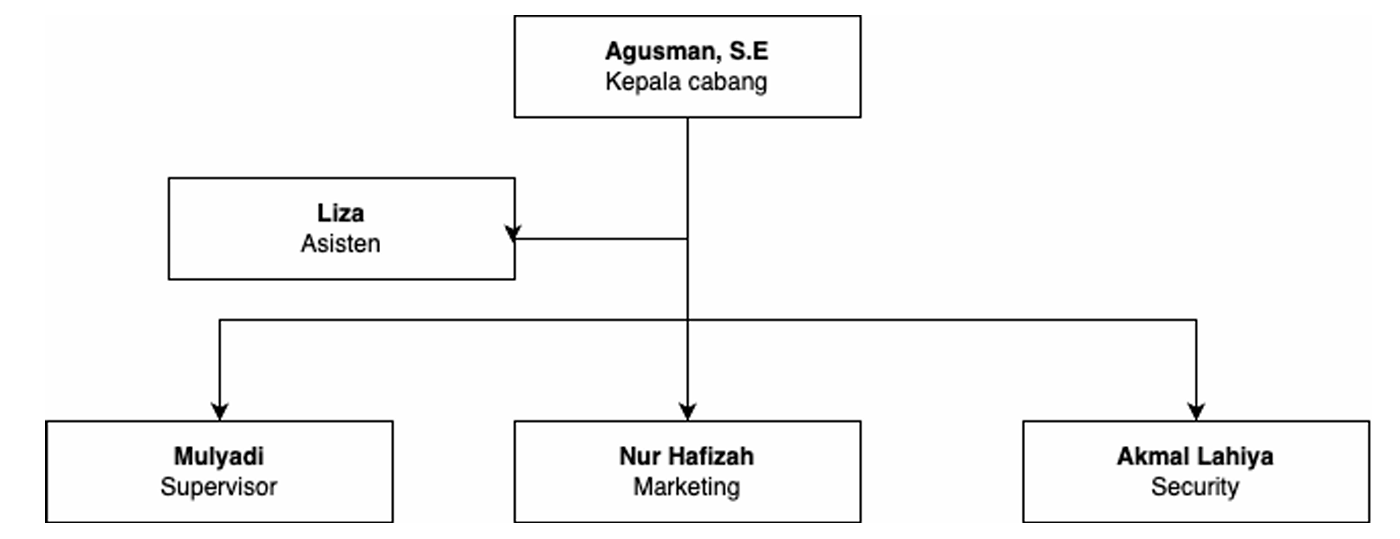
\includegraphics[width=0.75\linewidth]{Struktur Organisasi.png}
    \caption{Struktur Organisasi}
\end{figure}
% -----------------------------------------------------------------------------%
\section{Sistem}
% -----------------------------------------------------------------------------%
Menurut Azhar Susanto dalam bukunya yang berjudul Sistem Informasi Akuntansi: Sistem adalah kumpulan/group dari sub sistem/bagian/komponen apapun baik phisik ataupun non phisik yang saling berhubungan satu sama lain dan bekerja sama secara harmonis untuk mencapai satu tujuan tertentu. Sementara Mohamad Subhan dalam bukunya yang berjudul Analisa Perancangan Sistem mendefinisikan pengertian dari sistem sebagai berikut: Suatu sistem dapat diartikan sebagai suatu kumpulan atau himpunan dari unsur, komponen, atau variabel-variabel yang terorganisasi, saling berinteraksi, saling tergantung satu sama lain dan terpadu. Sistem juga merupakan kumpulan elemen-elemen saling terkait dan bekerja sama untuk memproses masukan (input) yang ditujukan kepada sistem tersebut dan mengolah masukan tersebut sampai menghasilkan keluaran (output) yang diinginkan. Berdasarkan beberapa pendapat yang dikemukakan di atas dapat ditarik kesimpulan bahwa sistem adalah kumpulan bagian-bagian atau sub-sub sistem yang disatukan dan dirancang untuk mencapai suatu tujuan. (Wibawa, 2017).

% -----------------------------------------------------------------------------%
\section{Informasi}
Informasi adalah hasil pemrosesan data yang diperoleh dari setiap elemen sistem tersebut menjadi bentuk yang mudah dipahami dan merupakan pengetahuan yang relevan yang dibutuhkan oleh setiap orang untuk menambah pemahamannya terhadap fakta-fakta yang ada. Informasi bagi setiap elemen akan berbeda satu sama lain sesuai dengan kebutuhannya masing-masing. Ada beberapa definisi informasi menurut para ahli, yakni Menurut (Jogiyanto, 2005), informasi dapat didefinisikan   sebagai data yang diolah menjadi bentuk  yang lebih  berguna  dan  lebih  berarti  bagi yang menerimanya. (Zaliluddin, 2020)
% -----------------------------------------------------------------------------%
\section{Sistem Informasi}
% -----------------------------------------------------------------------------%
Menurut McLeod (2009) Sistem Informasi merupakan sistem yang mempunyai kemampuan untuk mengumpulkan informasi dari semua sumber dan menggunakan berbagai media untuk menampilkan informasi. Menurut Sidharta (1995: 11), “Sebuah sistem informasi adalah sistem buatan manusia yang berisi himpunan terintegrasi dari komponen - komponen manual dan komponen - komponen terkomputerisasi yang bertujuan untuk mengumpulkan data, memproses data, dan menghasilkan informasi untuk pemakai”. Berdasarkan dari beberapa pendapat dapat disimpulkan sistem informasi dapat diartikan sebagai sebuah sistem yang terintegrasi secara optimal dan berbasis komputer yang dapat menghimpun dan menyajikan berbagai jenis data yang akurat untuk berbagai macam kebutuhan. (Firliana et al., 2018).
%-----------------------------------------------------------------------------%

\subsection{Siklus Sistem Informasi}
Siklus Sistem Informasi adalah data yang diolah melalui model menjadi informasi, penerima kemudian menerima informasi tersebut. Membuat suatu keputusan dan melakukan tindakan, yang berarti menghasilkan suatu tindakan yang lain yang akan membuat sejumlah data kembali. Data tersebut akan ditangkap sebagai input, diproses kembali lewat suatu model dan seterusnya membentuk suatu siklus. Siklus ini oleh John Burch disebut dengan siklus informasi \textit{(information cycle)} atau ada yang menyebutkan dengan istilah siklus pengolahan data \textit{(Data processing cycles)}.

\subsection{Komponen Sistem Informasi}
\par Adapun komponen sistem informasi yaitu sebagai berikut:

	\begin{enumerate}
	  	\item Komponen Input/Masukan.
			\par Input merupakan data yang masuk kedalam sistem informasi. Komponen ini merupakan bahan dasar dalam pengolahan informasi. Data untuk sistem informasi perlu ditangkap dan dicatat dalam dokumen dasar. Dokumen dasar merupakan formulir yang digunakan untuk menangkap (capture) dari data yang terjadi, yang selanjutnya data tersebut dimasukkan kedalam sistem informasi \textit{(data entry)}.
	 	 \item Komponen Model.
			\par Informasi yang dihasilkan oleh sistem informasi berasal dari data yang diambil dari basis data yang diolah melalui model-model tertentu.
		\item Komponen Output/Keluaran.
			\par Output adalah produk yang dihasilkan dari sitem informasi yang berguna bagi para pemakainya.
	 	 \item Komponen Teknologi.
			\par Komponen teknologi merupakan komponen penting dalam sistem informasi. Tanpa ada teknologi yang mendukung, maka sistem informasi tidak akan dapat menghasilkan informasi yang tepat waktu.
		\item Komponen Basis Data.
			\par Basis data \textit{(database)} adalah kumpulan dari data yang saling berhubungan satu dengan yang lainnya, tersimpan diperangkat keras komputer dan digunakan perangkat lunak untuk memanipulasinya.
	\end{enumerate}
%-----------------------------------------------------------------------------%
\section{Oktaax}
\par Oktaax merupakan pustaka PHP yang ringan dan dirancang untuk aplikasi berbasis event-driven, yang cocok digunakan untuk aplikasi dengan kebutuhan concurrency tinggi. Pustaka ini memungkinkan pengelolaan koneksi WebSocket secara efisien, mendukung pengembangan aplikasi dengan waktu respons yang cepat, serta mempermudah integrasi dalam server berbasis PHP. Keunggulan utama pustaka ini terletak pada kesederhanaannya dalam penggunaan, memungkinkan pengembangan yang lebih cepat tanpa mengorbankan performa, yang menjadikannya pilihan ideal untuk aplikasi real-time seperti dashboard interaktif \citep{rosyida2021swoole}.
%-----------------------------------------------------------------------------%
\section{Perumahan}
Berdasarkan Undang-undang Nomor 1 tahun 2011 tentang perumahan dan pemukiman. Perumahan adalah kelompok rumah yang berfungsi sebagai lingkungan tempat tinggal atau lingkungan hunian yang dilengkapi dengan sarana dan prasarana lingkungan.
\par Menurut Majalah Properti Indonesia (edisi tahun 2015-2019), konsep perumahan terdiri dari: 
\begin{enumerate}
\item \textit{Eco Living}, Konsep ini memiliki desain yang diatur sedemikian rupa, sehingga sirkulasi udara dan cahaya bisa leluasa.
\item \textit{Custom Homes}, konsep ini menawarkan hunian dengan desain yang dipilih oleh konsumen sesuai dengan selera dan budget.
\item \textit{Tropical Modern Landscape}, konsep ini dirancang dengan unit-unit hunian di dalam perumahan tidak saling menempel antara satu rumah dengan rumah lainnya, sehingga dapat menghadirkan ruang terbuka hijau di samping rumah sekaligus memberikan pencahayaan alami yang maksimal dan memberikan efek visual yang berbeda, 
\item \textit{Urban Smart and Livable}, konsep urban mengadopsi desain arsitektur minimalis.
\end{enumerate}
%-----------------------------------------------------------------------------%
\section{Model Perancangan \textit{Object Oriented Analysis Design} (\textit{OOAD}) }
Metode berorientasi objek atau object oriented merupakan paradigma baru dalam rekayasa perangkat lunak yang memandang sistem sebagai kumpulan objek - objek diskrit yang saling berinteraksi. Yang dimaksud dengan berorientasi objek adalah bahwa mengorganisasikan perangkat lunak sebagai kumpulan objek - objek diskrit yang bekerja sama antara informasi atau struktur data dan perilakau \textit{(behavior)} yang mengaturnya \citep{ariska2016rancang}.
%-----------------------------------------------------------------------------%
\section{\textit{Unified Modelling Language} (\textit{UML})}
Menurut (Sugiarti, 2018) adalah sebuah visualisasi, merancang dan mendokumentasikan sistem piranti lunak. Salah satu standar yang digunakan diperindustrian untuk mengetahui dan mendefinisakan requirement, analisis dan desain, dari suatu arsitektur dalam pemrograman berorientasi objek. (Wahyuni, 2022).
%-----------------------------------------------------------------------------%
\subsection{Diagram \textit{UML} Yang Digunakan}
%-----------------------------------------------------------------------------%
Berikut adalah diagram \textit{UML} yang akan digunakan dalam laporan kerja praktek.
\begin{enumerate}
    \item \textbf{\textit{Use Case Diagram}}\\ \textit{Use Case diagram} merupakan uraian sekelompok yang saling terkait dan membentuk sistem secara teratur yang dilakukan atau diawasi oleh sebuah aktor. \textit{Use Case} atau diagram use case merupakan pemodelan untuk melakukan \textit{(behavior)} sistem informasi yang akan dibuat. (Nuddin \& Fithri, 2015). Tujuan utama permodelan \textit{use case} adalah:

\begin{enumerate} [label=\alph*.]
\item Memutuskan dan mendiskripsikan kebutuhan-kebutuhan fungsional sistem.
\item Memberikan deskripsi jelas dan konsisten dari apa yang seharusnya dilakukan, sehingga model \textit{use case} digunakan diseluruh proses pengembangan untuk komunikasi dan menyediakan basis untuk pemodelan berikutnya yang mengacu sistem harus memberikan fungsionalitas yang dimodelkan para \textit{use case}.
\item Menyediakan basis untuk melakukan pengujian sistem yang memverifikasi sistem. Menguji apakah sistem telah memberikan fungsionalitas yang diminta.
\item Menyediakan kemampuan melacak kebutuhan fungsionalitas menjadi kelas-kelas dan operasi-operasi aktual di sistem. Untuk menyederhanakan perubahan dan ekstensi ke sistem dengan mengubah model use case dan kemudian melacak \textit{use case} yang dipengaruhi ke perancangan dan implementasi sistem.
\end{enumerate}

\par Syarat penamaan \textit{use case} adalah nama didefenisikan sesederhana mungkin dan dapat dipahami, ada dua hal utama pada \textit{use case} yaitu pendefenisian apa yang disebut aktor dan \textit{use case}.

\begin{enumerate} [label=\alph*.]
\item Aktor merupakan orang, proses, atau sistem lain yang berinteraksi dengan sistem informasi yang akan di buat diluar sistem informasi yang akan dibuat sendiri, jadi walaupun simbol dari aktor adalah gambar orang tapi aktor belum tentu orang.
\item  \textit{use case} merupakan fungsionalitas yang disediakan sistem sebagai unit-unit yang saling bertukar pesan antar unit atau aktor.
\end{enumerate}

\captionsetup{position=above} % Mengatur posisi caption di atas
\begin{small}
			\begin{longtable}[c]{|c|>{\centering\arraybackslash}m{2cm}|c|p{7.6cm}|}
			\caption{\textit{Simbol Use Case Diagram}} \label{tab:my-table}\\ % Caption di atas tabel
			\hline
			No & Gambar & Nama & Keterangan \\ \hline
			\endfirsthead
			%
			\endhead
			%
			1 & \parbox[c][2cm][c]{2cm}{\centering 
\includegraphics[height=1cm]{useCase/actor.jpg}} & \textit{Actor} & \textit{Use Case} menggambarkan fungsionalitas yang disediakan sistem sebagai unit-unit yang bertukar pesan antar unit dengan aktor, yang dinyatakan dengan menggunakan kata kerja \\ \hline
			
			2 & \raisebox{-.5\height}{
\includegraphics[width=1.5cm]{useCase/dependency.png}} & \textit{Dependency} & Hubungan dimana perubahan yang terjadi pada suatu elemen mandiri (\textit{independent}) akan mempengaruhi elemen yang bergantung padanya, elemen yang tidak mandiri (\textit{independent}). \\ \hline
			3 & \raisebox{-.5\height}{
\includegraphics[width=1.5cm]{useCase/generalization.jpg}} & \textit{Generalization} & Hubungan dimana objek anak (\textit{descendent}) berbagi perilaku dan struktur data dari objek yang ada di atasnya objek induk (\textit{ancestor}). \\ \hline
			4 & \raisebox{-.5\height}{
\includegraphics[width=1.5cm]{useCase/include.jpg}} & \textit{Include} & Menspesifikasikan bahwa \textit{use case} sumber secara eksplisit. \\ \hline
			5 & \raisebox{-.5\height}{
\includegraphics[width=1.5cm]{useCase/extend.png}} & \textit{Extend} & Menspesifikasikan bahwa \textit{use case} target memperluas perilaku dari use case sumber pada suatu titik yang diberikan. \\ \hline
			6 & \raisebox{-.5\height}{
\includegraphics[width=1.5cm]{useCase/association.png}} & \textit{Association} & Apa yang menghubungkan antara objek satu dengan objek lainnya. \\ \hline
			7 & \raisebox{-.5\height}{
\includegraphics[width=1cm, height=1cm]{useCase/system.png}} & \textit{System} & Menspesifikasikan paket yang menampilkan sistem secara terbatas. \\ \hline
			8 & \raisebox{-.5\height}{
\includegraphics[width=1.5cm]{useCase/use case.jpg}} & \textit{Use Case} & Deskripsi dari urutan aksi-aksi yang ditampilkan sistem yang menghasilkan. \\ \hline
			\end{longtable}
			\end{small}

        \item  \textbf{\textit{Activity Diagram}}\\ \textit{Activity diagram} menggambarkan aliran fungsionalitas dalam suatu sistem informasi. Secara lengkap, \textit{activity diagram} mendefinisikan dimana \textit{workflow} dimulai, dimana berhentinya, aktifitas apa yang terjadi selama \textit{workflow}, dan bagaimana urutan kejadian aktifitas tersebut \citep{dicoding2021activity}. \textit{Activity diagram} juga menyediakan pendekatan untuk proses pemodelan paralel. Bagi mereka yang akrab dengan analisis dan desain struktur tradisional, diagram ini menggabungkan ide-ide yang mendasari diagram alir data dan diagram alur sistem. (Dewi et al., 2012). 

		\par Diagram aktivitas berguna untuk sebagai berikut:
			
			\begin{enumerate} [label=\alph*.]
			\item Rancangan proses bisnis dimana setiap urutan aktivitas yang digambarkan merupakan proses bisnis sistem yang didefenisikan.
			\item Urutan atau pengelompokan tampilan dari sistem atau \textit{user interface} dimana setiap aktivitas di anggap memiliki sebuah rancangan antar muka tampilan.
			\item Rancangan tampilan dimana setiap aktivitas dianggap memerlukan sebuah pengujian yang perlu di defenisikan kasus ujinya.
			\end{enumerate}
        
\begin{small}     
		\begin{longtable}[c]{|c|>{\centering\arraybackslash}m{2cm}|c|p{8cm}|}
		    \captionsetup{position=above} % Menempatkan caption di atas tabel
		    \caption{Simbol \textit{Activity Diagram}} \label{tab:activity-diagram} \\ \hline
		    \textbf{No} & \textbf{Gambar} & \textbf{Nama} & \textbf{Keterangan} \\ \hline
		    \endfirsthead
		    % Tidak ada header lagi di halaman berikutnya
		    \endhead
		    \hline
		    \endfoot
		    % Konten tabel
		    1 & \parbox[c][1.5cm][c]{1.5cm}{\centering 
\includegraphics[width=1.5cm]{activityDiagram/activity.jpg}} & \textit{Activity} & Memperlihatkan bagaimana masing-masing kelas antar muka saling berinteraksi satu sama lain \\ \hline
		    2 & \parbox[c][1.5cm][c]{1.5cm}{\centering 
\includegraphics[width=1.5cm]{activityDiagram/action.jpg}} & \textit{Action} & State dari sistem yang mencerminkan eksekusi dari suatu aksi \\ \hline
		    3 & \parbox[c][2cm][c]{2cm}{\centering 
\includegraphics[width=1.5cm]{activityDiagram/initial node.png}} & \textit{Initial Node} & Bagaimana objek dibentuk atau diawali \\ \hline
		    4 & \parbox[c][2cm][c]{2cm}{\centering 
\includegraphics[width=1.5cm]{activityDiagram/activity final node.png}} & \textit{Final Node} & Bagaimana objek dibentuk dan dihancurkan \\ \hline
		    5 & \parbox[c][1.5cm][c]{1.5cm}{\centering 
\includegraphics[width=1.5cm]{activityDiagram/fork node.jpg}} & \textit{Fork Node} & Satu aliran yang pada tahap tertentu berubah menjadi beberapa aliran \\ \hline
		\end{longtable}
		\end{small}

    \item \textbf{\textit{Class Diagram}}\\ \textit{Class diagram} adalah salah satu pemodelan yang cukup penting dalam UML, fungsinya adalah untuk membuat sebuat \textit{logical models} dari sebuah sistem \citep{setiawan2021class}. Sebuah class diagram akan menunjukan bagaimana skema dari arsitektur sebuah sistem yang sedang dirancang (Kendal, 2009). \textit{Class diagram} digambarkan dengan class yang berisi atribut dan method, setiap class akan dihubungkan dengan sebuah garis disebut Asosiasi. \citep{aliman2021perancangan}. 
    
\begin{small} % Mengecilkan ukuran font tabel
	\begin{longtable}{|c|>{\centering\arraybackslash}m{2cm}|c|p{7.2cm}|}
	    \captionsetup{position=above} % Menempatkan caption di atas tabel
	    \caption{Simbol \textit{Class Diagram}} \label{tab:Class-Diagram} \\ \hline
	    \textbf{No} & \textbf{Gambar} & \textbf{Nama} & \textbf{Keterangan} \\ \hline
	    \endfirsthead
	    \textbf{No} & \textbf{Gambar} & \textbf{Nama} & \textbf{Keterangan} \\ \hline
	    \endhead
	    \hline
	    \endfoot
	    % Konten tabel
	    1 & \parbox[c][2cm][c]{2cm}{\centering 
\includegraphics[width=1.5cm, height=1cm]{classDiagram/generalization.jpg}} & \textit{Generalization} & Hubungan dimana objek anak (descendent) berbagi perilaku dan struktur data dari objek yang ada di atasnya, yaitu objek induk (ancestor). \\ \hline
	    2 & \parbox[c][2cm][c]{2cm}{\centering 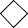
\includegraphics[width=1.5cm]{classDiagram/nary association.png}} & \textit{Nary Association} & Upaya untuk menghindari asosiasi dengan lebih dari dua objek. \\ \hline
	    3 & \parbox[c][2cm][c]{2cm}{\centering 
\includegraphics[width=1.5cm]{classDiagram/collaboration.png}} & \textit{Collaboration} & Deskripsi dari urutan aksi-aksi yang ditampilkan sistem, yang menghasilkan suatu hasil yang terukur bagi suatu aktor. \\ \hline
	    4 & \parbox[c][2cm][c]{2cm}{\centering 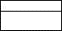
\includegraphics[width=1.5cm]{classDiagram/class.png}} & \textit{Class} & Himpunan dari objek-objek yang berbagi atribut serta operasi yang sama. \\ \hline
	    5 & \parbox[c][2cm][c]{2cm}{\centering 
\includegraphics[width=1.5cm]{classDiagram/realization.jpg}} & \textit{Realization} & Operasi yang benar-benar dilakukan oleh suatu objek. \\ \hline
	    6 & \parbox[c][2cm][c]{2cm}{\centering 
\includegraphics[width=1.5cm]{classDiagram/dependency.jpg}} & \textit{Dependency} & Hubungan dimana perubahan yang terjadi pada suatu elemen mandiri (independent) akan memengaruhi elemen yang bergantung. \\ \hline
	\end{longtable}
	\end{small}

\end{enumerate}
% -----------------------------------------------------------------------------%

\section{Metode \textit{Extreme Programming (XP)}}
% -----------------------------------------------------------------------------%
\par Penelitian ini menggunakan metode pengembangan sistem \textit{Extreme Programming (XP)}. Metode ini cocok untuk pengerjaan perangkat lunak, karena sifat dari metode ini sendiri dilakukan dengan cepat dan juga cenderung menggunakan pendekatan berorientasi objek dan sasaran dari tim yang dibentuk dalam skala kecil melalui tahapan-tahapan yang meliputi Planning (perencanaan), Design (perancangan), Coding (pengkodean), Testing (pengujian) \citep{andriani2023extreme}. 
\textit{Extreme Programming (XP)} merupakan sebuah metode pengembangan perangkat lunak yang mencoba meningkatkan efisiensi dan fleksibilitas dalam suatu pengembangan perangkat lunak yang mengombinasikan berbagai ide sederhana tanpa mengurangi kualitas software yang akan dibangun (Sri Ramadhani dkk., 2019).

\par Adapun tahapan dalam metode \textit{Extreme Programming (XP)} yaitu:

		\begin{enumerate}
			\item \textit{Planning}
			\par Pada tahapan ini merupakan tahapan awal dalam pembangunan sistem dimana dalam tahapan ini dilakukan beberapa kegiatan perencanaan, yaitu, identifikasi permasalahan, menganalisa kebutuhan, sampai dengan penetapan jadwal pelaksanaan pembangunan sistem (Septiani \& Yanti, t.t.).
			\item \textit{Design}
			\par Pada tahapan ini merupakan tahapan perancangan dengan melakukan kegiatan pemodelan yang dimulai dari pemodelan sistem, pemodelan arsitektur sampai dengan pemodelan basis data (Septiani \& Habibie, 2022).
			\item \textit{Coding}
			\par Pada tahapan ini merupakan kegiatan penerapan pemodelan yang sudah dibuat dalam bentuk user interface, dengan menggunakan bahasa pemrograman (Risma dkk., 2021).
			\item \textit{Testing}
			\par Setelah tahapan pengkodean berhasil diselesaikan, kemudian tahapan selanjutnya adalah tahapan pengujian sistem untuk mengetahui kesalahan apa saja yang timbul saat aplikasi sedang berjalan serta mengetahui apakah sistem yang dibangun sudah sesuai dengan kebutuhan pengguna (Marta Syakira, 2022).
		\end{enumerate}
% -----------------------------------------------------------------------------%
%-----------------------------------------------------------------------------------------------%
%
% % Oktober 2022
% Template Latex untuk Laporan Kerja Praktek Program Studi Sistem informasi ini
% Dikembangkan oleh Daffa Takratama Savra (daffatakratama13@gmail.com)

% Template ini dikembangkan dari template yang dibuat oleh Inggih Permana (inggihjava@gmail.com).

% Orang yang cerdas adalah orang yang paling banyak mengingat kematian.
%
%-----------------------------------------------------------------------------------------------%


%-----------------------------------------------------------------------------%
\chapter{\babTiga}
%-----------------------------------------------------------------------------%
\section{Waktu dan Tempat Pelaksaan Kerja Praktek}
Adapun waktu dan tempat pelaksanaan kegiatan kerja praktek ini adalah sebagai berikut:
\par Tanggal           : 01 September 2024 – 30 September 2024 
\par Waktu Kerja    : Senin – Jum’at (08.00 – 15.00)
\par Tempat            : Perumahan Kamala Permai


%-----------------------------------------------------------------------------%
\subsection{Jadwal Kerja Praktek}
Berikut adalah jadwal pelaksanaan kerja praktek ini terhitung 1 bulan (30 hari), seperti pada tabel 3.1 dibawah ini:
%-----------------------------------------------------------------------------%

\begin{table}[H]
\centering
\captionsetup{position=above} % Menempatkan caption di atas tabel
\caption{Jadwal Kerja Praktek}
\begin{tabular}{|c|c|c|c|c|}
\hline
\multirow{2}{*}{\textbf{Jenis Kegiatan}} & \multicolumn{4}{c|}{\textbf{Minggu Ke-}} \\ \cline{2-5} 
                                         & \textbf{I} & \textbf{II} & \textbf{III} & \textbf{IV} \\ \hline
Pengenalan dengan lingkungan kerja        & \cellcolor[HTML]{3166FF} & \cellcolor[HTML]{FFFFFF} & \cellcolor[HTML]{FFFFFF} & \cellcolor[HTML]{FFFFFF} \\ \hline
Pengumpulan data                          & \cellcolor[HTML]{3166FF} & \cellcolor[HTML]{3166FF} & \cellcolor[HTML]{FFFFFF} & \cellcolor[HTML]{FFFFFF} \\ \hline
Analisa dan perancangan sistem            & \cellcolor[HTML]{FFFFFF} & \cellcolor[HTML]{3166FF} & \cellcolor[HTML]{3166FF} & \cellcolor[HTML]{FFFFFF} \\ \hline
Implementasi sistem                       & \cellcolor[HTML]{FFFFFF} & \cellcolor[HTML]{FFFFFF} & \cellcolor[HTML]{3166FF} & \cellcolor[HTML]{3166FF} \\ \hline
Penyusunan laporan                        & \cellcolor[HTML]{FFFFFF} & \cellcolor[HTML]{FFFFFF} & \cellcolor[HTML]{FFFFFF} & \cellcolor[HTML]{3166FF} \\ \hline
\end{tabular}
\end{table}

\subsection{Uraian Kerja Praktek}
%-----------------------------------------------------------------------------%
Tugas Kerja Praktek ini dikerjakan di Perumahan Kamela Permai yang beralamatkan di Taluk Kuantan, Kec. Kuantan Tengah, Kab. Kuantan Singingi dalam kurun waktu 30 hari dihitung sejak 1 September s/d 31 September 2024. Kegiatan yang dilakukan disusun dalam proses perencanaan kerja, rencana tersebut adalah:
\begin{enumerate}
    \item Kegiatan pada minggu pertama dilakukan agenda proses perkenalan dengan tempat kerja. Perkenalan dilakukan pada tanggal 1 September 2024 mulai dari memperkenalkan diri kepada para pegawai. Perkenalan ini juga sekaligus berlangsung dengan pengumpulan data, yaitu dengan melakukan teknik pengumpulan seperti observasi dan wawancara.
    \item Pada Minggu kedua dilakukan proses pengamatan alur dan prosedur kerja, identifikasi tugas, khususnya di bidang bagian umum. Sekaligus memulai untuk menganalisa serta merancang sistem yang akan dibuat.
    \item  Pada minggu ketiga dilakukannya pengimplementasian sistem bersama pihak instansi.
    \item  Selanjutnya pada minggu keempat yaitu melakukan penyusunan laporan yang berasal dari data yang sudah diperoleh.
\end{enumerate}
%-----------------------------------------------------------------------------%
\section{Menentukan Data Yang Diperlukan}
\par Adapun data yang dikumpulkan pada saat kerja praktek adalah sebagai berikut:

\begin{enumerate} [label=\alph*.]
\item Data Primer
\par Data Primer adalah data yang diambil secara langsung dari sumber aslinya, melalui narasumber yang tepat dan dapat dijadikan data pembuatan laporan. Data primer tersebut adalah:
	\begin {enumerate}
	\item Daftar harga rumah setiap tipenya.
	\item Lokasi dan \textit{siteplan} untuk membuat visual digital
	\end{enumerate}
\item Sekunder
\par Data Sekunder adalah data yang diambil melalui jurnal, e-book dan juga buku-buku referensi dari berbagai penulis.
\end{enumerate}
%-----------------------------------------------------------------------------%
%-----------------------------------------------------------------------------%
\section{Metodologi Kerja Praktek}
%-----------------------------------------------------------------------------%
\begin{figure}
    \centering
    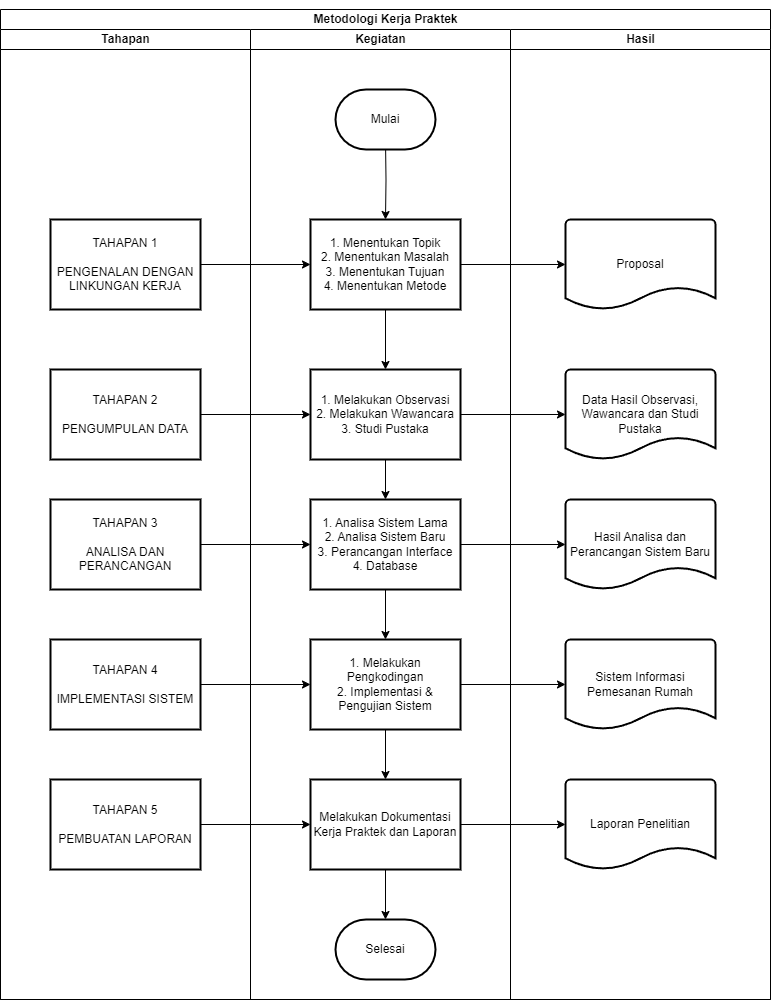
\includegraphics[width=\textwidth]{Flowchart Metodologi Kerja Praktek.png}
    \caption{Metodologi Kerja Praktek}
    \label{fig:enter-label}
\end{figure}
%-----------------------------------------------------------------------------%
\subsection{Tahap Pengenalan dengan Lingkungan Kerja}
%-----------------------------------------------------------------------------%
\par Langkah Pertama adalah perkenalan dengan lingkungan instansi sekaligus menetapkan masalah yang akan dipecahkan dalam instansi tersebut. Adapun langkah-langkah dalam tahap ini adalah sebagai berikut:

\begin{enumerate}
    \item Mulai\\Merupakan tahapan awal dalam setiap kegiatan yang akan dilakukan. 
    \item Menentukan Topik Penelitian\\Topik penelitian ditentukan dari uraian masalah dan kendala yang didapat dari observasi secara langsung di Perumahan Kamela Permai.
 \item Menentukan Masalah\\Setelah observasi dilakukan untuk mendukung pencapaian kerja praktek maka selanjutnya dilakukan penentuan masalah agar bisa mendapat masalah yang lebih fokus untuk dipecahkan. 
    \item Menentukan Tujuan Kerja Praktek\\Selanjutnya adalah penentuan tujuan dari kerja praktek ini agar tujuan dalam penulisan Laporan Kerja Praktek lebih Jelas. 
 \item Menentukan Metode Penelitian\\Agar hasil dari penelitian ini sesuai harapan maka dibutuhkan penentuan metode penelitian untuk mendukung penelitian ini. 
\end{enumerate}
%-----------------------------------------------------------------------------%
\subsection{Tahap Pengumpulan Data}
%-----------------------------------------------------------------------------%
\par Tahap ini adalah tahap penulis melaksanakan Kerja Praktek, pada tahap ini yang dilakukan adalah:

\begin{enumerate}
    \item Observasi\\Penulis melakukan pengamatan di Perumahan Kamela Permai secara langsung juga melakukan peninjauan di Perumahan Kamela Permai. 
    \item Wawancara\\Penulis melakukan wawancara langsung dengan marketing Perumahan Kamela Permai terkait pemesanan perumahan. 
    \item Studi Pustaka\\Studi Pustaka dilakukan dengan cara mengambil literature yang berkaitan dengan materi. Pada tahapan pengumpulan data studi pustaka penulis mengambil beberapa referensi dari buku, jurnal, e-book dan internet.
\end{enumerate}
%-----------------------------------------------------------------------------%
\subsection{Tahap Analisa dan Perancangan}
%-----------------------------------------------------------------------------%
\par Beberapa hal yang perlu dilakukan dalam tahap analisa dan perancangan sistem adalah sebagai berikut:

\begin{enumerate}
	    \item Analisa Sistem Lama\\Pada tahap analisa sistem lama atau sistem yang berjalan, penulis melihat langsung bagaimana proses pemesanan berlangsung dimana calon pembeli akan datang ke kantor pemasaran dan merencanakan pemesanan serta menanyakana dokumen yang perlu disiapkan. 
	    \item Analisa Sistem Baru\\Pada tahap analisa sistem baru penulis mengambil usulan berdasarkan masalah dan kendala yang sudah dilakukan di analisa sistem yang berjalan (sistem lama), sehingga penulis mempunyai usulan sistem baru berupa:
			\begin{enumerate} 
			\item Penyimpanan data setiap rumah beserta type dan harganya menggunakan database
			\item Pencarian data untuk mengurangi penumpukan data.
			\end{enumerate}
	    \item Perancangan \textit{Interface}\\Pada tahap ini penulis membuat perencangan interface yang merupakan desain dari fitur yang telah diusulkan pada analisa sistem baru yang menghasilkan perancangan sebagai berikut:
	\begin{enumerate} [label=\alph*.]
		\item Perancangan \textit{interface} halaman \textit{home}.
		\item Perancangan \textit{interface} halaman \textit{siteplan} untuk pemesanan.
		\item Perancangan \textit{interface} halaman data rumah.
		\item Perancangan \textit{interface} halaman data pengunjung.
		\item Perancangan \textit{interface} halaman panduan pemesanan.
		\item Perancangan \textit{interface} halaman \textit{gallery}.
		\item Perancangan \textit{interface} halaman harga.
		\item Perancangan \textit{interface} halaman kontak.
		\item Perancangan \textit{interface} halaman \textit{login}
		\item Perancangan \textit{interface} halaman \textit{booking}
		\item Perancangan \textit{interface} halaman \textit{Dashboard}
	\end{enumerate}
	\item \textit{Database}\\Pada tahap ini penulis melakukan rancangan database berdasarkan perancangan interface yang telah ditentukan yaitu membuat struktur \textit{tabel, record, field} dan \textit{ERD}.
\end{enumerate}
%-----------------------------------------------------------------------------%
\subsection{Tahap Implementasi}
%-----------------------------------------------------------------------------%
Dalam tahap pembuatan sistem informasi absensi pegawai ini terdapat pengodingan dan pendesain web. Yaitu dengan menggunakan bahasa pemrograman \textit{PHP} dengan menggunakan \textit{HTTP Library Oktaax} dan \textit{MySQL} sebagai \textit{Database}. Implementasi Sistem yaitu tahap dimana sistem siap dioperasikan pada keadaan yang sebenarnya sesuai dari kebutuhan dari perumahan, sehingga dapat diketahui sistem yang dibuat benar-benar dapat memecahkan masalah yang ada.
%-----------------------------------------------------------------------------%
\subsection{Tahap Penulisan Laporan}
%-----------------------------------------------------------------------------%
\par Tahap terakhir adalah melakukan penyusunan laporan. Kegiatan yang dilakukan diantaranya melakukan konsultasi terhadap pembimbing kerja praktek, melakukan dokumentasi hasil kerja praktek, dan selesai.
\par Penelitian sebagai bahan dari laporan kerja praktek ini dilakukan dengan menggunakan penelitian deskriptif yaitu metode penelitian yang bertujuan menggambarkan secara sistematis dan akurat mengenai data-data yang ada dengan cara mengumpulkan dan mengklasifikasikan data yang diperoleh, kemudian dianalisis dengan teori yang telah dipelajari.
%-----------------------------------------------------------------------------%

\ifthenelse{\equal{\bidangta}{DUA}}{
  \renewcommand{\babEmpat}{ANALISIS DAN HASIL}
  \renewcommand{\babLima}{PENUTUP}
}{}

\ifthenelse{\equal{\tipeta}{LAPORAN KERJA PRAKTEK}}{
  \renewcommand{\babEmpat}{ANALISA DAN HASIL}
}{}

%-----------------------------------------------------------------------------------------------%
%
% % Oktober 2022
% Template Latex untuk Laporan Kerja Praktek Program Studi Sistem informasi ini
% Dikembangkan oleh Daffa Takratama Savra (daffatakratama13@gmail.com)

% Template ini dikembangkan dari template yang dibuat oleh Inggih Permana (inggihjava@gmail.com).

% Orang yang cerdas adalah orang yang paling banyak mengingat kematian.
%
%-----------------------------------------------------------------------------------------------%


%-----------------------------------------------------------------------------%
\chapter{\babEmpat}
% -----------------------------------------------------------------------------%
\section{Analisa Sistem}
\par Analisa sistem adalah penguraian dari suatu sistem informasi yang utuh ke dalam bagian-bagian komponennya dengan maksud tujuan untuk mengidentifikasikan dan mengevaluasi permasalahan-permasalahan yang diharapkan, sehingga dapat di usulkan perbaikan-perbaikannya. Sebelum melakukan analisis sistem, terlebih dahulu harus mengetahui dan memahami sistem, dan diperlukannya data dari sistem untuk dianalisa, yaitu hal-hal yang berkenaan dengan definisi data tersebut.
% -----------------------------------------------------------------------------%
\subsection{Analisa Sistem Yang Sedang Berjalan}
% -----------------------------------------------------------------------------%
Pada tahap analisa sistem lama atau sistem yang berjalan, penulis melihat langsung bagaimana proses pemesanan berlangsung dimana calon pembeli akan datang ke kantor pemasaran dan merencanakan pemesanan serta menanyakan dokumen yang perlu disiapkan. Lalu dari pihak marketing akan memprosess dokumen yang diberikan oleh calon pembeli.
\par Berikut adalah uraian dari sistem yang sedang berjalan pada  Pemesanan Rumah di Perumahan Kamela Permai: 
\begin{enumerate}
    \item Tamu Menanyakan Syarat Pemesanan: Proses dimulai dengan tamu yang ingin melakukan pemesanan, bertanya kepada staff mengenai syarat-syarat yang diperlukan.
    \item Staff Memberikan Formulir Pemesanan: Staff memberikan formulir pemesanan kepada tamu untuk diisi. Formulir ini berisi informasi yang harus dilengkapi oleh tamu agar dapat memproses pemesanan.
    \item Tamu Mengisi Formulir: Tamu mengisi formulir pemesanan yang diberikan oleh staff dengan data-data yang diperlukan.
    \item Tamu Membuat Pemesanan (Credit/Cash): Setelah mengisi formulir, tamu memilih metode pembayaran, apakah secara kredit atau tunai.
    \item Staff Memeriksa Dokumen Syarat Pemesanan: Staff memeriksa apakah dokumen yang diserahkan oleh tamu memenuhi syarat pemesanan atau tidak.
    \item Keputusan Dokumen Memenuhi: Jika dokumen memenuhi syarat, maka staff melanjutkan ke proses selanjutnya. Jika tidak, tamu mungkin diminta untuk melengkapi dokumen atau mengisi ulang formulir.
    \item Memproses Dokumen Pemesanan: Setelah dokumen dinyatakan lengkap, staff memproses dokumen pemesanan sesuai prosedur yang berlaku.
    \item Proses pemesanan selesai setelah dokumen diproses.
\end{enumerate}

\par Adapun analisa sistem yang sedang berjalan pada Pemesanan Rumah di Perumahan Kamela Permai dapat dilihat pada Gambar 4.1 berikut:
\begin{figure}
\centering
    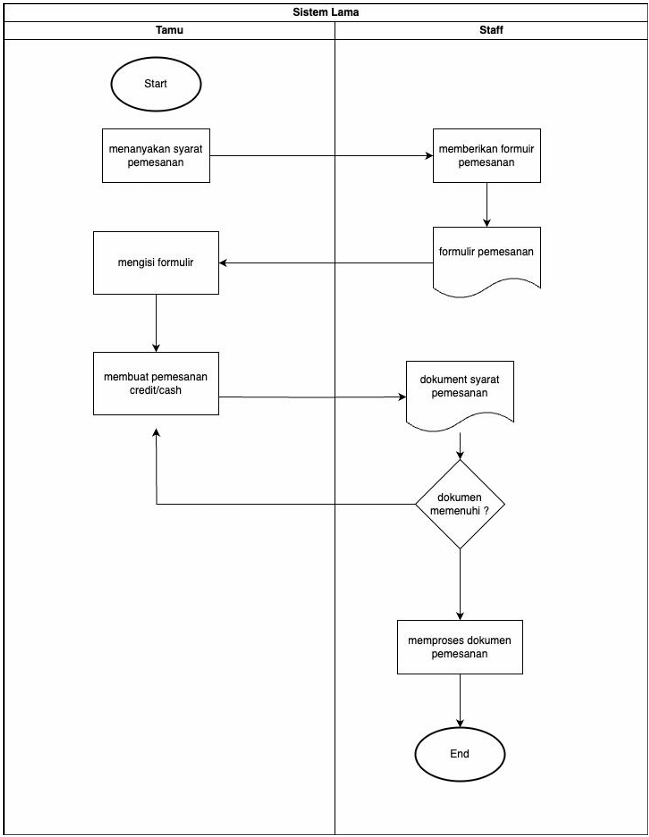
\includegraphics[width=0.90\linewidth]{Analisa sistem yang sedang berjalan.png}
    \caption{Analisa Sistem Yang Sedang Berjalan}
\end{figure}
% -----------------------------------------------------------------------------%
\section{Analisa Sistem Yang Diusulkan}
% -----------------------------------------------------------------------------%
\par Berdasarkan hasil analisa sistem yang sedang berjalan, proses seperti itu membuat proses pemesanan berjalan lama, dan sulit ditangani jika terdapat lebih dari 1 pemesan dalam satu waktu. Oleh karena itu, dibutuhkanlah sebuah sistem yang dapat digunakan oleh pengelola Perumahan Kamela permai dalam menangani proses pemesanan yang terkomputerisasi, dengan membuat sebuah sistem pemesanan berbasis web. Dimana proses pemesanan hanya dilakukan menggunaan smartphone/laptop.
\par Dalam Sistem  sudah terdapat panduan bagaimana dan apa syarat untuk memesan sebuah ruman di Perumahan Kamela Permai. Data calon  akan langsung tersimpan didalam sistem sehingga pengelola hanya perlu mengunggu data tersebut masuk berapa pun banyaknya.
\par Adapun analisa sistem yang diusulkan penulis dapat dilihat pada Gambar 4.2 berikut:
\begin{figure}
\centering
    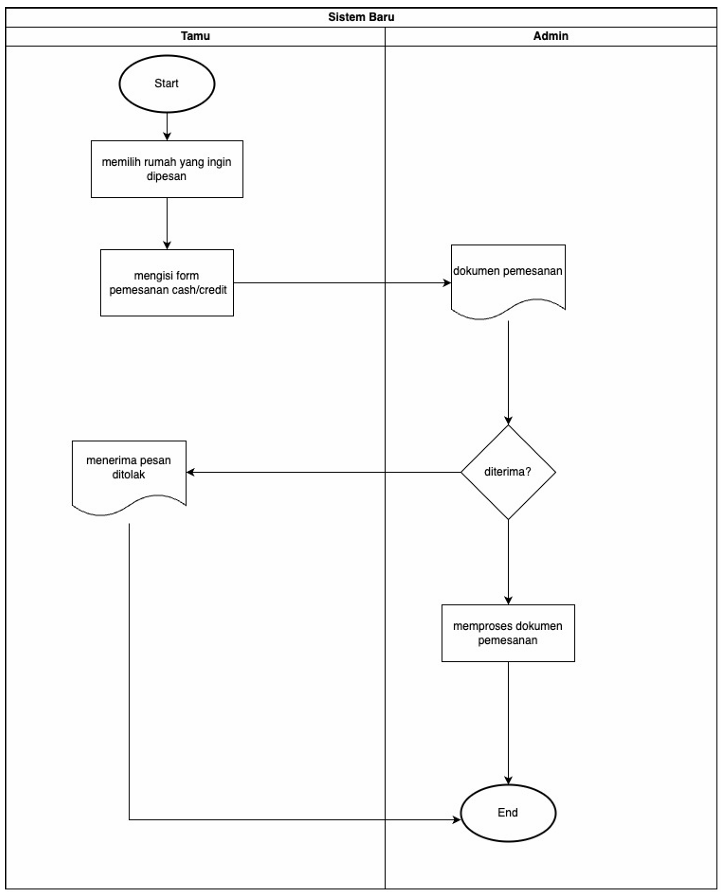
\includegraphics[width=0.90\linewidth]{Analisa Sistem Yang Diusulkan.png}
    \caption{Analisa Sistem Yang Diusulkan}
\end{figure}
% -----------------------------------------------------------------------------%
\subsection{Rencana Sistem Usulan}
% -----------------------------------------------------------------------------%
\subsection{\textit{Use Case Diagram}}
% -----------------------------------------------------------------------------%
\par Use Case Diagram terdiri dari \textit{Actor, Use Case} dan serta hubungannya. \textit{Use Case Diagram} adalah sesuatu yang penting untuk memvisualisasikan, menspesifikasikan dan mendokumentasikan kebutuhan perilaku sistem. \textit{Use Case Diagram} digunakan untuk menjelaskan kegiatan apa saja yang dapat dilakukan oleh \textit{user} pada sistem yang sedang berjalan. Penggambaran sistem dalam bentuk \textit{use case} dapat dilihat pada Gambar 4.3 berikut:
\begin{figure}
    \centering
    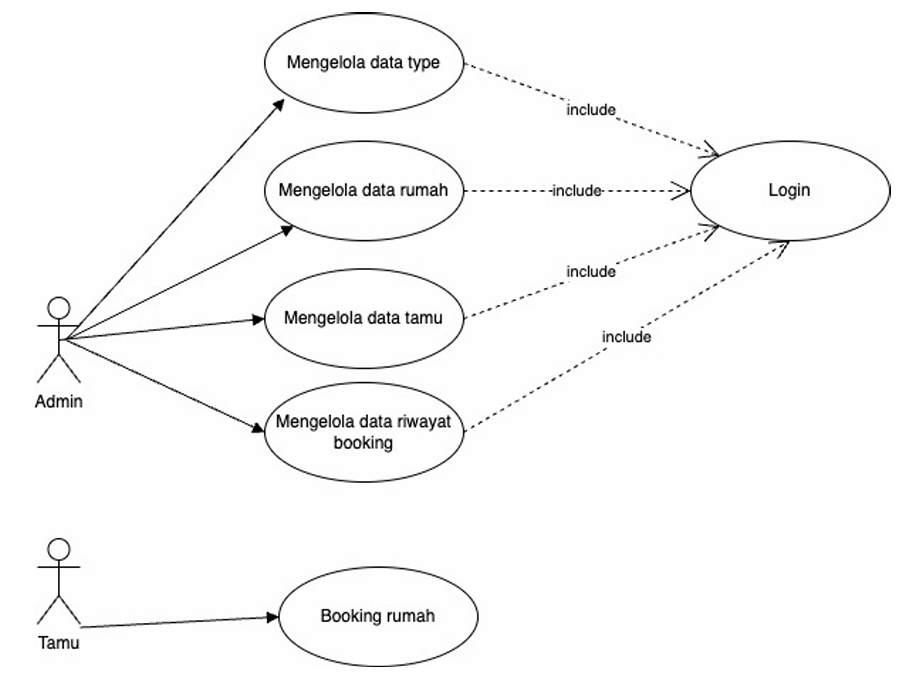
\includegraphics[width=1.0\linewidth]{Use Case Diagram.png}
    \caption{\textit{Use Case Diagram}}
    \label{fig:enter-label}
\end{figure}


    \par Adapun penjelasan mengenai aktor-aktor pada use case diagram sistem yang usulan ini dapat dilihat pada tabel berikut:

\begin{longtable}[c]{|l|l|p{9cm}|} % Gunakan p{10cm} agar teks panjang dibungkus
\captionsetup{position=above} % Menempatkan caption di atas tabel
\caption{Deskripsi Aktor}
\label{tab:my-table}\\
\hline
Aktor & Sinonim          & Deskripsi                                                                                                                                                                                      \\ \hline
\endfirsthead
% Kosongkan untuk menghilangkan teks "continued from previous page"
\endhead
%
Admin  & \textit{Administrator}             & Orang / Bagian yang bertugas mengelola data tamu, rumah type rumah didalam sistem.                                      \\ \hline
Tamu  & \textit{Guest}     & Tamu adalah calon pelanggan yang bisa merupakan siapa saja dan dapat memesan perumahan di Perumahan Kamela Permai.                                                                                                                   \\ \hline
\end{longtable}

\par Berikut ini merupakan deskripsi dari masing-masing \textit{use case} yang berada pada Sistem Informasi Pemesanan Perumahan Kamela Permai.
\begin{longtable}[c]{|l|l|p{9cm}|} % Gunakan p{10cm} agar teks panjang dibungkus
\captionsetup{position=above} % Menempatkan caption di atas tabel
\caption{Deskripsi \textit{Use Case} Diagram}
\label{tab:my-table}\\
\hline
No & \textit{Use Case}          & Deskripsi                                                                                                                                                                                      \\ \hline
\endfirsthead
% Kosongkan untuk menghilangkan teks "continued from previous page"
\endhead
%
1  & Login             & \textit{Use Case} ini menggambarkan aktor masuk ke sistem dengan menggunakan \textit{username} dan \textit{password}.                                      \\ \hline
2  & Kelola Data Rumah     & \textit{Use Case} ini menggambarkan admin dapat mengelola data, antara lain; mengubah status dan mengedit blok dan nomor rumah.                                                                                                                   \\ \hline
3  & Kelola Data Tamu         & \textit{Use Case} ini menggambarkan admin dapat mengubah status, melihat data yang diinputkan tamu serte menghapus data tamu.                                                                            \\ \hline
4  & Kelola Data riwayat    & \textit{Use Case} ini menggambarkan admin dapat mengelola data Riwayat Tamu yang berhasil memesan rumah lewat sistem.               \\ \hline
5  & Booking    & \textit{Use Case} ini menggambarkan tamu dapat memesan dengan memilih salah satu rumah dan memanginputkan data yang diperlukan. \\ \hline
\end{longtable}

\begin{enumerate}
    \item Skenario\textit{ Use Case Diagram}
\par Skenario \textit{use case} menyatakan urutan pesan dan tindakan tunggal yang ada pada sistem. Berikut ditampilkan skenario use case dari setiap use case yang telah ada.
\end{enumerate}
\begin{enumerate}[label=\alph*.]
    \item Skenario \textit{Use Case Login}
	\par Skenario \textit{Use Case Login} dapat dilihat pada tabel berikut:

        \begin{longtable}{|p{5cm}|p{9cm}|}
	    \caption{Skenario \textit{Use Case Login}}
	    \label{tab:my-table} \\ \hline
	    \multicolumn{1}{|c|}{\textbf{Komponen}} & \multicolumn{1}{c|}{\textbf{Deskripsi}} \\ \hline
	    \endfirsthead
	    \hline
	    \multicolumn{1}{|c|}{\textbf{Komponen}} & \multicolumn{1}{c|}{\textbf{Deskripsi}} \\ \hline
	    \endhead
	    Nama \textit{Use Case} & \textit{Login} \\ \hline
	    Deskripsi & \textit{Use case} ini menggambarkan \textit{actor} masuk ke sistem dengan menggunakan \textit{username} dan \textit{password}. \\ \hline
	    Aktor & Admin \\ \hline
	    \textit{Pre-Condition} & Sistem menampilkan halaman \textit{login}. \\ \hline
	    \textit{Post-Condition} & Aktor berhasil \textit{login}. \\ \hline
	    \multicolumn{2}{|c|}{\textbf{Skenario Normal}} \\ \hline
	    \multicolumn{1}{|c|}{\textbf{Aksi Aktor}} & \multicolumn{1}{c|}{\textbf{Reaksi Sistem}} \\ \hline
	    1. Aktor melakukan \textit{login} dengan menginput \textit{username} dan \textit{password} & \\ \hline
	    & 2. Sistem melakukan verifikasi \textit{login}. \\ \hline
	    & 3. Sistem menampilkan \textit{form} menu utama. \\ \hline
	    \multicolumn{2}{|c|}{\textbf{Skenario Gagal}} \\ \hline
	    \multicolumn{1}{|c|}{\textbf{Aksi Aktor}} & \multicolumn{1}{c|}{\textbf{Reaksi Sistem}} \\ \hline
	    1. Aktor melakukan \textit{login} dengan menginput \textit{username} dan \textit{password} & \\ \hline
	    & 2. Sistem melakukan verifikasi \textit{login}. \\ \hline
	    & 3. Sistem menampilkan pesan gagal login karena kredensial tidak valid. \\ \hline
	\end{longtable}


    
    \item Skenario \textit{Use Case} Kelola Data Rumah
	\par Skenario \textit{Use Case} Kelola Data Rumah dapat dilihat pada tabel berikut:

       \begin{longtable}{|p{5cm}|p{9cm}|}
	    \caption{Skenario \textit{Use Case} Kelola Data Rumah}
	    \label{tab:my-table} \\ \hline
	    \multicolumn{1}{|c|}{\textbf{Komponen}} & \multicolumn{1}{c|}{\textbf{Deskripsi}} \\ \hline
	    \endfirsthead
	    \endhead
	    Nama \textit{Use Case} & Kelola Data Rumah \\ \hline
	    Deskripsi & \textit{Use case} ini menggambarkan actor dapat mengubah data rumah \\ \hline
	    Aktor & Admin \\ \hline
	    \textit{Pre-Condition} & Sistem memasuki halaman data rumah. \\ \hline
	    \textit{Post-Condition} & Sistem menampilkan halaman data rumah. \\ \hline
	    \multicolumn{2}{|c|}{\textbf{Skenario Normal}} \\ \hline
	    \multicolumn{1}{|c|}{\textbf{Aksi Aktor}} & \multicolumn{1}{c|}{\textbf{Reaksi Sistem}} \\ \hline
	    1. Aktor masuk ke halaman data rumah & \\ \hline
	    & 2. Sistem menampilkan halaman data rumah \\ \hline
	    3. Aktor melihat, mengubah nomor/blok dan status rumah & \\ \hline
	    & 4. Sistem menyimpan perubahan data rumah \\ \hline
	    \multicolumn{2}{|c|}{\textbf{Skenario Alternatif: Gagal}} \\ \hline
	    \multicolumn{1}{|c|}{\textbf{Aksi Aktor}} & \multicolumn{1}{c|}{\textbf{Reaksi Sistem}} \\ \hline
	    1. Admin menuju halaman keuangan & \\ \hline
	    & 2. Sistem menampilkan halaman data pegawai \\ \hline
	    3. Aktor melihat, mengubah nomor/blok dan status rumah & \\ \hline
	    & 4. Sistem menampilkan pesan gagal menyimpan penambahan atau perubahan data rumah \\ \hline
	\end{longtable}

        
    \item Skenario \textit{Use Case} Kelola Data Tamu
	\par Skenario \textit{Use Case} Kelola Data Tamu dapat dilihat pada tabel berikut:

    \begin{longtable}{|p{5cm}|p{9cm}|}
	    \caption{Skenario \textit{Use Case} Kelola Data Tamu}
	    \label{tab:my-table} \\ \hline
	    \multicolumn{1}{|c|}{\textbf{Komponen}} & \multicolumn{1}{c|}{\textbf{Deskripsi}} \\ \hline
	    \endfirsthead
	    \endhead
	    Nama \textit{Use Case} & Kelola Data Tamu \\ \hline
	    Deskripsi & \textit{Use case} ini menggambarkan aktor dapat mengelola data tamu antara lain; menerima pesanan tamu dan menghapus tamu \\ \hline
	    Aktor & Admin \\ \hline
	    \textit{Pre-Condition} & Sistem memasuki halaman tamu. \\ \hline
	    \textit{Post-Condition} & Sistem menampilkan halaman tamu. \\ \hline
	    \multicolumn{2}{|c|}{\textbf{Skenario Normal}} \\ \hline
	    \multicolumn{1}{|c|}{\textbf{Aksi Aktor}} & \multicolumn{1}{c|}{\textbf{Reaksi Sistem}} \\ \hline
	    1. Aktor masuk ke halaman tamu & \\ \hline
	    & 2. Sistem menampilkan halaman data tamu \\ \hline
	    3. Aktor melihat, mengubah dan menghapus data tamu & \\ \hline
	    & 4. Sistem mengubah atau menghapus data tamu \\ \hline
	    \multicolumn{2}{|c|}{\textbf{Skenario Alternatif: Gagal}} \\ \hline
	    \multicolumn{1}{|c|}{\textbf{Aksi Aktor}} & \multicolumn{1}{c|}{\textbf{Reaksi Sistem}} \\ \hline
	    1. Aktor masuk ke halaman data jabatan & \\ \hline
	    & 2. Sistem menampilkan halaman data jabatan \\ \hline
	    3. Aktor melihat, mengubah, dan menghapus data tamu & \\ \hline
	    & 4. Sistem menampilkan pesan gagal menyimpan pengubahan atau penghapusan data tamu \\ \hline
	\end{longtable}
     
    
    \item Skenario \textit{Use Case Booking}
    
	\par Skenario \textit{Use Case Booking} dapat dilihat pada tabel berikut:

        \begin{longtable}{|p{5cm}|p{9cm}|}
	    \caption{Skenario \textit{Use Case} Booking}
	    \label{tab:my-table} \\ \hline
	    \multicolumn{1}{|c|}{\textbf{Komponen}} & \multicolumn{1}{c|}{\textbf{Deskripsi}} \\ \hline
	    \endfirsthead
	    \endhead
	    Nama \textit{Use Case} & Booking \\ \hline
	    Deskripsi & \textit{Use case} ini menggambarkan aktor dapat membuat pemesanan rumah. \\ \hline
	    Aktor & Tamu \\ \hline
	    \textit{Pre-Condition} & Sistem memasuki halaman \textit{siteplan}. \\ \hline
	    \textit{Post-Condition} & Sistem menampilkan halaman \textit{siteplan}. \\ \hline
	    \multicolumn{2}{|c|}{\textbf{Skenario Normal}} \\ \hline
	    \multicolumn{1}{|c|}{\textbf{Aksi Aktor}} & \multicolumn{1}{c|}{\textbf{Reaksi Sistem}} \\ \hline
	    1. Aktor masuk ke halaman \textit{siteplan} & \\ \hline
	    & 2. Sistem menampilkan \textit{siteplan} \\ \hline
	    3. Aktor melihat dan memilih rumah untuk dipesan & \\ \hline
	    & 4. Sistem menampilkan opsi metode kredit atau tunai \\ \hline
	    5. Aktor memilih metode & \\ \hline
	    & 6. Sistem memberikan halaman formulir untuk pemesanan \\ \hline
	    7. Aktor mengisi formulir & \\ \hline
	    & 8. Sistem menyimpan data dan memberikan pesan berhasil \\ \hline
	    \multicolumn{2}{|c|}{\textbf{Skenario Alternatif: Gagal}} \\ \hline
	    \multicolumn{1}{|c|}{\textbf{Aksi Aktor}} & \multicolumn{1}{c|}{\textbf{Reaksi Sistem}} \\ \hline
	    1. Aktor memilih rumah yang telah dipesan oleh orang lain & \\ \hline
	    & 2. Sistem menampilkan pesan gagal karena rumah tidak tersedia \\ \hline
	    3. Aktor mencoba mengisi formulir dengan data yang tidak valid & \\ \hline
	    & 4. Sistem menampilkan pesan gagal menyimpan data pemesanan \\ \hline
	\end{longtable}
    
    
    \item Skenario \textit{Use Case} Kelola \textit{Type}

\par Skenario \textit{Use Case} Kelola \textit{Type} dapat dilihat pada tabel berikut.
        
        \begin{longtable}{|p{5cm}|p{9cm}|}
	    \captionsetup{position=above} % Menempatkan caption di atas tabel
	    \caption{Skenario \textit{Use Case} Kelola Data Tamu}
	    \label{tab:my-table} \\ \hline
	    \multicolumn{1}{|c|}{\textbf{Komponen}} & \multicolumn{1}{c|}{\textbf{Deskripsi}} \\ \hline
	    \endfirsthead
	    \endhead
	    Nama \textit{Use Case} & Kelola \textit{Type} \\ \hline
	    Deskripsi & \textit{Use case} ini menggambarkan aktor dapat menambah atau menghapus gambar serta mengganti harga untuk tiap \textit{Type}. \\ \hline
	    Aktor & Admin \\ \hline
	    \textit{Pre-Condition} & Sistem memasuki halaman data \textit{Type}. \\ \hline
	    \textit{Post-Condition} & Sistem menampilkan halaman data \textit{Type}. \\ \hline
	    \multicolumn{2}{|c|}{\textbf{Skenario Normal}} \\ \hline
	    \multicolumn{1}{|c|}{\textbf{Aksi Aktor}} & \multicolumn{1}{c|}{\textbf{Reaksi Sistem}} \\ \hline
	    1. Aktor masuk ke halaman data \textit{Type} & \\ \hline
	    & 2. Sistem menampilkan halaman data \textit{Type} \\ \hline
	    3. Aktor melihat, menambah, mengubah, dan menghapus data \textit{Type} & \\ \hline
	    & 4. Sistem menyimpan penambahan, pengubahan, atau pengapusan data \textit{Type} \\ \hline
	    \multicolumn{2}{|c|}{\textbf{Skenario Alternatif: Gagal}} \\ \hline
	    \multicolumn{1}{|c|}{\textbf{Aksi Aktor}} & \multicolumn{1}{c|}{\textbf{Reaksi Sistem}} \\ \hline
	    1. Aktor masuk ke halaman data type & \\ \hline
	    & 2. Sistem menampilkan halaman data \textit{Type} \\ \hline
	    3. Aktor melihat, menambah, mengubah dan menghapus data \textit{Type} & \\ \hline
	    & 4. Sistem menampilkan pesan gagal menyimpan penambahan, pengubahan atau pengapusan data \textit{Type} \\ \hline
	\end{longtable}
  
        
    \item Skenario \textit{Use Case} Kelola Data Riwayat
	
	\par Skenario \textit{Use Case} Kelola Riwayat dapat dilihat pada tabel berikut.

        \begin{longtable}{|p{5cm}|p{9cm}|}
	    \captionsetup{position=above} % Menempatkan caption di atas tabel
	    \caption{Skenario \textit{Use Case} Kelola Data Riwayat}
	    \label{tab:my-table} \\ \hline
	    \multicolumn{1}{|c|}{\textbf{Komponen}} & \multicolumn{1}{c|}{\textbf{Deskripsi}} \\ \hline
	    \endfirsthead
	    \endhead
	    Nama \textit{Use Case} & Kelola Data Riwayat \\ \hline
	    Deskripsi & \textit{Use case} ini menggambarkan aktor dapat melihat atau menghapus data riwayat pemesanan yang berhasil. \\ \hline
	    Aktor & Admin \\ \hline
	    Kondisi Awal & Sistem memasuki halaman data riwayat \\ \hline
	    Kondisi Akhir & Sistem menampilkan halaman data riwayat \\ \hline
	    \multicolumn{2}{|c|}{\textbf{Skenario Normal}} \\ \hline
	    \multicolumn{1}{|c|}{\textbf{Aksi Aktor}} & \multicolumn{1}{c|}{\textbf{Reaksi Sistem}} \\ \hline
	    1. Aktor masuk ke halaman data riwayat & \\ \hline
	    & 2. Sistem menampilkan halaman data riwayat \\ \hline
	    3. Aktor melihat dan menghapus data riwayat & \\ \hline
	    & 4. Sistem menghapus data riwayat \\ \hline
	    \multicolumn{2}{|c|}{\textbf{Skenario Alternatif: Gagal}} \\ \hline
	    \multicolumn{1}{|c|}{\textbf{Aksi Aktor}} & \multicolumn{1}{c|}{\textbf{Reaksi Sistem}} \\ \hline
	    1. Aktor masuk ke halaman data riwayat & \\ \hline
	    & 2. Sistem menampilkan halaman data riwayat \\ \hline
	    3. Aktor melihat, menambah, mengubah dan menghapus data \textit{type} & \\ \hline
	    & 4. Sistem menampilkan pesan gagal penghapusan data \textit{type}, kesalahan sistem pada \textit{database}. \\ \hline
	\end{longtable}

    
\end{enumerate}
% -----------------------------------------------------------------------------%
\subsection{\textit{Activity Diagram}}
% -----------------------------------------------------------------------------%
\par Diagram aktivitas menggambarkan aliran fungsionalitas sistem yang dapat digunakan untuk menunjukkan aliran kejadian \textit{(Flow of events)} dalam \textit{use case}. Setiap proses yang terjadi dalam sistem akan digambarkan secara rinci dan lengkap, dengan langkah demi langkahnya mulai dari masukan hingga keluaran.
\par Proses sistem Pemesanan Rumah di Perumahan Kamela Permai yang diusulkan ini akan dijelaskan pada Activity Diagram berikut:

\begin{enumerate}
    \item \textit{Activity Diagram Login}
        \par \textit{Activity Diagram Login } dapat dilihat dari gambar berikut:
            \begin{figure}
                \centering
                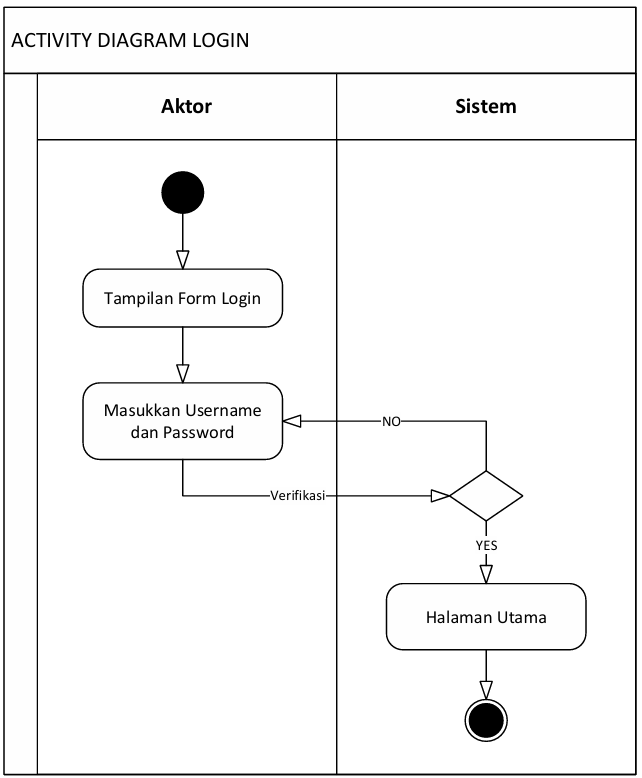
\includegraphics[width=0.95\linewidth]{uml/Activity Diagram - Login.png}
                \caption{\textit{Activity Diagram} Login}
                \label{fig:enter-label}
            \end{figure}
            
    \item \textit{Activity Diagram} Kelola Rumah
        \par \textit{Activity Diagram} Kelola Rumah dapat dilihat dari gambar berikut:
            \begin{figure}
                \centering
                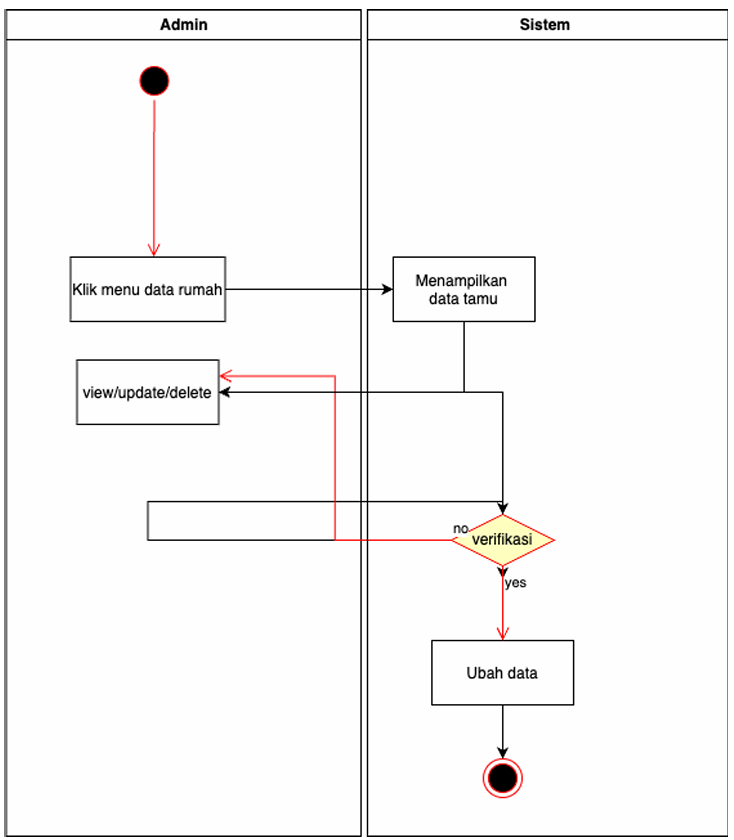
\includegraphics[width=0.95\linewidth]{uml/Activity Diagram - Kelola Rumah.png}
                \caption{\textit{Activity Diagram} Kelola Rumah}
                \label{fig:enter-label}
            \end{figure}
	
	\item \textit{Activity Diagram} Kelola Data Tamu
        \par \textit{Activity Diagram} Kelola Data Tamu dapat dilihat dari gambar berikut:
            \begin{figure}
                \centering
                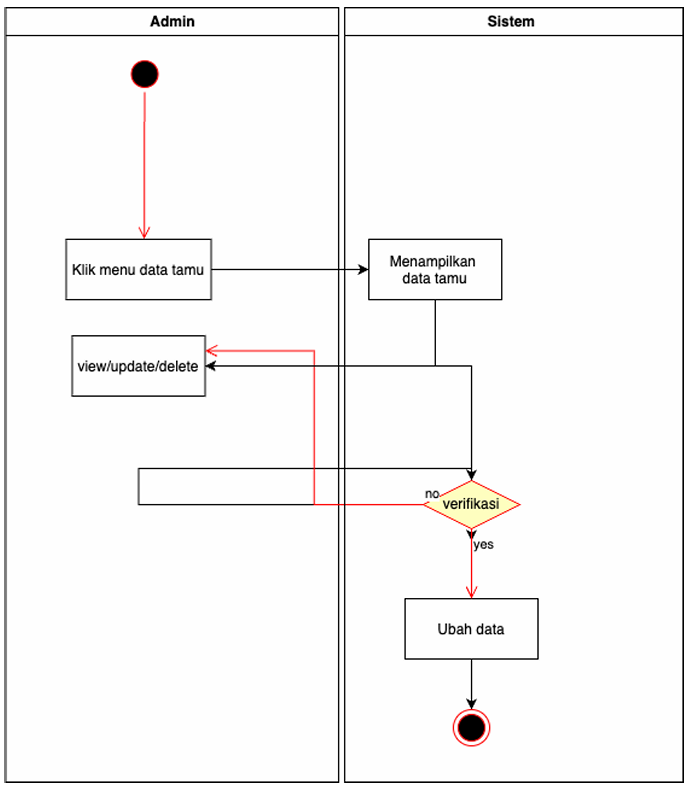
\includegraphics[width=0.95\linewidth]{uml/Activity Diagram - Kelola Tamu.png}
                \caption{\textit{Activity Diagram} Kelola Data Tamu}
            \end{figure}

    \item \textit{Activity Diagram} Kelola Data \textit{Type}
        \par \textit{Activity Diagram} Kelola Data \textit{Type} dapat dilihat dari gambar berikut:
            \begin{figure}
                \centering
                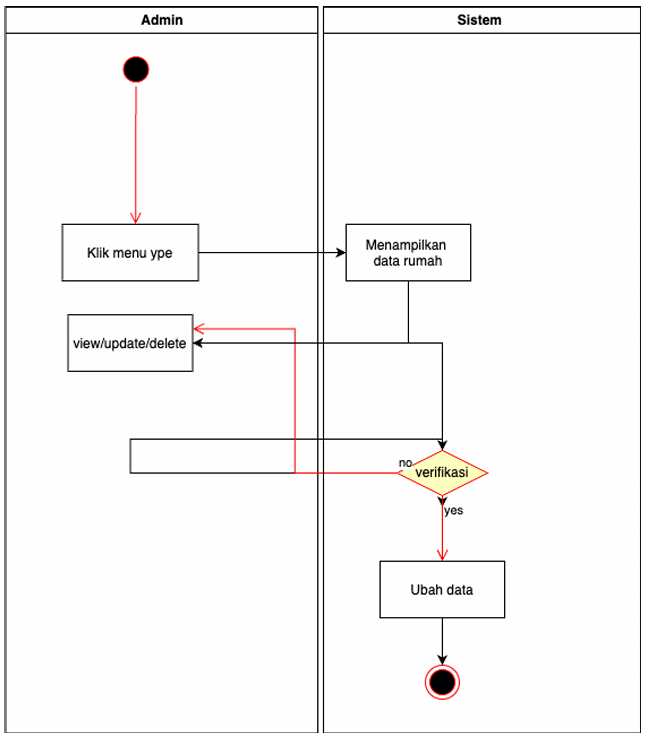
\includegraphics[width=0.95\linewidth]{uml/Activity Diagram - Kelola Type.png}
                \caption{\textit{Activity Diagram} Kelola Data \textit{Type}}
                \label{fig:enter-label}
            \end{figure}
    \item \textit{Activity Diagram Booking}
        \par \textit{Activity Diagram Booking} dapat dilihat dari gambar berikut:
            \begin{figure}
                \centering
                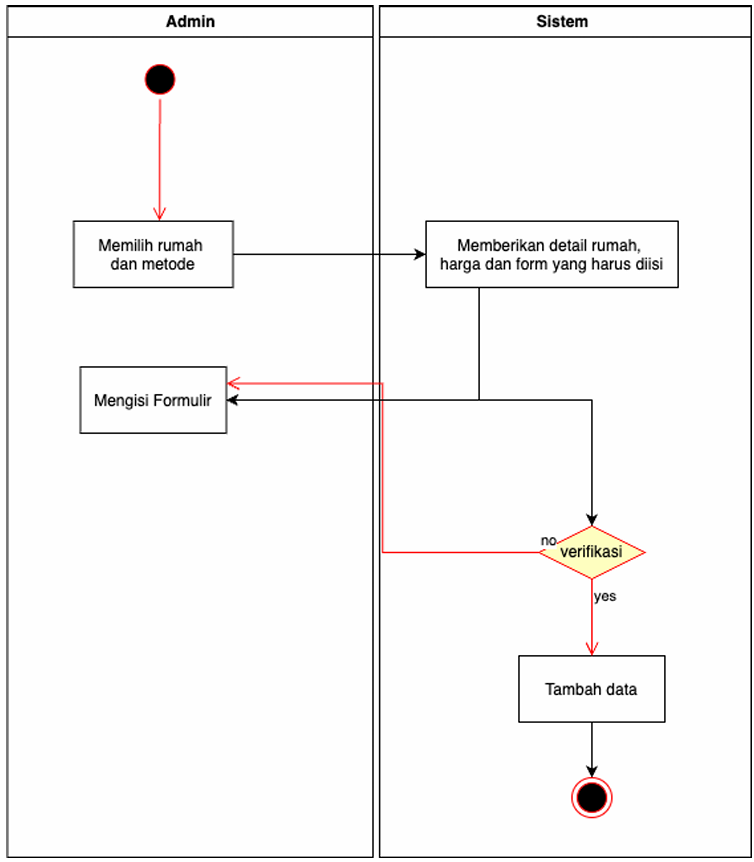
\includegraphics[width=0.95\linewidth]{uml/Activity Diagram - Booking.png}
                \caption{\textit{Activity Diagram Booking}}
                \label{fig:enter-label}
            \end{figure}
\end{enumerate}

% -----------------------------------------------------------------------------%
\subsection{\textit{Class Diagram}}
% -----------------------------------------------------------------------------%
\par \textit{Class Diagram} amerupakan diagram yang menunjukkan beberapa \textit{class} yang ada pada sistem serta hubungannya secara logic. \textit{Class Diagram} yang dibuat pada tahap design ini, merupakan deskripsi lengkap dari \textit{class-class} yang ditangani oleh sistem, dimana masing-masing \textit{class} telah dilengkapi dengan atribut dan operasi-operasi yang diperlukan.
\par Adapun \textit{Class Diagram} pada sistem yang diusulkan ini dapat dilihat pada gambar berikut:

\begin{figure}
    \centering
    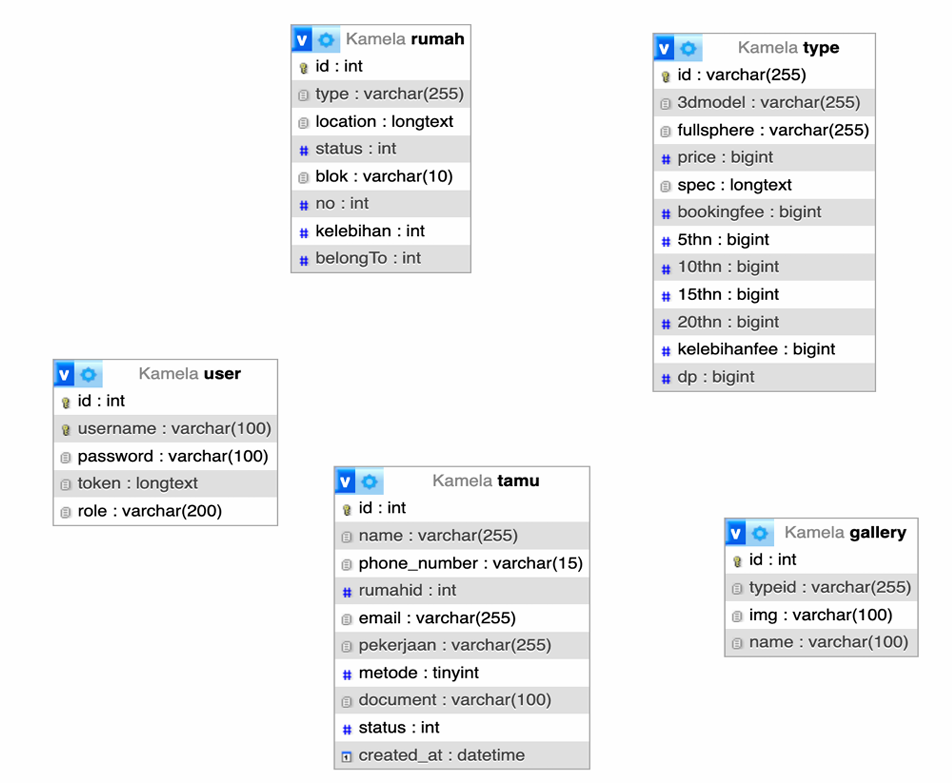
\includegraphics[width=0.95\linewidth]{Class Diagram.png}
    \caption{\textit{Class Diagram}}
\end{figure}

% -----------------------------------------------------------------------------%
\subsection{Perancangan \textit{Database}}
% -----------------------------------------------------------------------------%
\par Pada perancangan \textit{database} terdapat beberapa tabel yang saling berelasi. Perancangan \textit{database} yang akan digunakan pada sistem, didasari oleh data instansi. Perancangan ini bertujuan agar field data yang memiliki relasi dapat terhubung pada tabel di \textit{database}, sehingga proses pengaksesan data akan terorganisir dengan lebih baik.

\par Berikut adalah detail perancangan serta relasi yang ada pada \textit{database} sistem informasi pemesanan perumahan:

\begin{enumerate}
    \item \textbf{Tabel Absen}
    
    \begin{itemize}
        \item Nama Tabel: Users
        \item \textit{Primary Key}: id
    \end{itemize}

   \begin{longtable}{|p{5cm}|p{3cm}|p{2cm}|p{3cm}|}
	    \captionsetup{position=above} % Menempatkan caption di atas tabel
	    \caption{Tabel Struktur Database User}
	    \label{tab:struktur-database} \\ \hline
	    \multicolumn{1}{|c|}{\textbf{Nama Field}} & \multicolumn{1}{c|}{\textbf{Type}} & \multicolumn{1}{c|}{\textbf{Null}} & \multicolumn{1}{c|}{\textbf{Default}} \\ \hline
	    \endfirsthead
	    \hline
	    \multicolumn{1}{|c|}{\textbf{Nama Field}} & \multicolumn{1}{c|}{\textbf{Type}} & \multicolumn{1}{c|}{\textbf{Null}} & \multicolumn{1}{c|}{\textbf{Default}} \\ \hline
	    \endhead
	    id & int(11) & No & \\ \hline
	    username & varchar(255) & No & \\ \hline
	    password & varchar(255) & No & \\ \hline
	    token & varchar(255) & Yes & \\ \hline
	    role & varchar(255) & No & \\ \hline
	\end{longtable}


    \item \textbf{Tabel Type}

    \begin{itemize}
        \item Nama Tabel: Type
        \item \textit{Primary Key}: id
    \end{itemize}

     \begin{longtable}{|p{5cm}|p{3cm}|p{2cm}|p{3cm}|}
	    \captionsetup{position=above} % Menempatkan caption di atas tabel
	    \caption{Tabel Struktur Type}
	    \label{tab:struktur-database} \\ \hline
	    \multicolumn{1}{|c|}{\textbf{Column}} & \multicolumn{1}{c|}{\textbf{Type}} & \multicolumn{1}{c|}{\textbf{Null}} & \multicolumn{1}{c|}{\textbf{Default}} \\ \hline
	    \endfirsthead
	    \hline
	    \multicolumn{1}{|c|}{\textbf{Column}} & \multicolumn{1}{c|}{\textbf{Type}} & \multicolumn{1}{c|}{\textbf{Null}} & \multicolumn{1}{c|}{\textbf{Default}} \\ \hline
	    \endhead
	    id & varchar(255) & No & \\ \hline
	    3dmodel & varchar(255) & No & \\ \hline
	    price & bigInt & No & \\ \hline
	    spec & json & No & \\ \hline
	    bookingfee & bigInt & No & \\ \hline
		dp & bigInt & No & \\ \hline
		5thn & bigInt & Yes & \\ \hline
		10thn & bigInt & Yes & \\ \hline
		15thn & bigInt & Yes & \\ \hline
		20thn & bigInt & Yes & \\ \hline
		additionalfee & bigInt & Yes & \\ \hline
	\end{longtable}

    \item \textbf{Tabel House}
    
    \begin{itemize}
        \item Nama Tabel: house
        \item \textit{Primary Key}: id
    \end{itemize}
    
    \begin{longtable}{|p{5cm}|p{3cm}|p{2cm}|p{3cm}|}
	    \captionsetup{position=above} % Menempatkan caption di atas tabel
	    \caption{Tabel Struktur House}
	    \label{tab:struktur-database} \\ \hline
	    \multicolumn{1}{|c|}{\textbf{Column}} & \multicolumn{1}{c|}{\textbf{Type}} & \multicolumn{1}{c|}{\textbf{Null}} & \multicolumn{1}{c|}{\textbf{Default}} \\ \hline
	    \endfirsthead
	    \hline
	    \multicolumn{1}{|c|}{\textbf{Column}} & \multicolumn{1}{c|}{\textbf{Type}} & \multicolumn{1}{c|}{\textbf{Null}} & \multicolumn{1}{c|}{\textbf{Default}} \\ \hline
	    \endhead
	    id & int(11) & No & \\ \hline
	    type & varchar(255) & No & \\ \hline
	    location & varchar(255) & No & \\ \hline
	    status & int(3) & Yes & \\ \hline
	    blok & varchar(255) & No & \\ \hline
		no & int(3) & No & \\ \hline
		additional & int(255) & Yes & \\ \hline
		belongTo & int(11) & Yes & \\ \hline
	\end{longtable}

    \item \textbf{Tabel Guest}
    
    \begin{itemize}
        \item Nama Tabel: guest
        \item \textit{Primary Key}: id
    \end{itemize}

   \begin{longtable}{|p{5cm}|p{3cm}|p{2cm}|p{3cm}|}
	    \captionsetup{position=above} % Menempatkan caption di atas tabel
	    \caption{Tabel Guest}
	    \label{tab:struktur-database} \\ \hline
	    \multicolumn{1}{|c|}{\textbf{Column}} & \multicolumn{1}{c|}{\textbf{Type}} & \multicolumn{1}{c|}{\textbf{Null}} & \multicolumn{1}{c|}{\textbf{Default}} \\ \hline
	    \endfirsthead
	    \hline
	    \multicolumn{1}{|c|}{\textbf{Column}} & \multicolumn{1}{c|}{\textbf{Type}} & \multicolumn{1}{c|}{\textbf{Null}} & \multicolumn{1}{c|}{\textbf{Default}} \\ \hline
	    \endhead
	    id & int(11) & No & \\ \hline
	    name & varchar(50) & No & \\ \hline
	    phone\_number &	varchar(15) & No & \\ \hline
	    house\_id & int(11) & No & \\ \hline
	    email & varchar(50) & No & \\ \hline
		job & varchar(50) & No & \\ \hline
		method & tinyInt & No & \\ \hline
		document & varchar(50) & No & \\ \hline
		status & int(11) & No & \\ \hline
		created\_at & date & No & current\_datetime \\ \hline
	\end{longtable}

    \item \textbf{Tabel Gallery}
    
    \begin{itemize}
        \item Nama Tabel: Gallery
        \item \textit{Primary Key}: id
    \end{itemize}

    \begin{longtable}{|p{5cm}|p{3cm}|p{2cm}|p{3cm}|}
	    \captionsetup{position=above} % Menempatkan caption di atas tabel
	    \caption{Tabel Struktur Database Gallery}
	    \label{tab:struktur-database} \\ \hline
	    \multicolumn{1}{|c|}{\textbf{Nama Field}} & \multicolumn{1}{c|}{\textbf{Type}} & \multicolumn{1}{c|}{\textbf{Null}} & \multicolumn{1}{c|}{\textbf{Default}} \\ \hline
	    \endfirsthead
	    \hline
	    \multicolumn{1}{|c|}{\textbf{Nama Field}} & \multicolumn{1}{c|}{\textbf{Type}} & \multicolumn{1}{c|}{\textbf{Null}} & \multicolumn{1}{c|}{\textbf{Default}} \\ \hline
	    \endhead
	    id & int(11) & No & \\ \hline
	    typeid & varchar(11) & No & \\ \hline
	    name & varchar(255) & Yes & \\ \hline
	    image & varchar(255) & No & \\ \hline
	\end{longtable}

\end{enumerate}
% -----------------------------------------------------------------------------%
\subsection{Perancangan\textit{ Interface}}
% -----------------------------------------------------------------------------%
\par Perancangan antarmuka pengguna merupakan suatu proses yang kompleks, hal ini didasari karena antarmuka pengguna merupakan bagian dari sistem yang akan dikendalikan oleh pengguna dan merupakan tahap persiapan untuk rancang bangun implementasi. Oleh karena itu, untuk mendapatkan sistem yang dapat berjalan sesuai dengan fungsi yang diharapkan, diperlukannya pengalaman dalam merancang antarmuka pengguna, kreativitas yang tinggi, analisis tugas dan dapat menyesuaikan dengan kebutuhan serta kemampuan pengguna.

    \begin{enumerate}
        \item Perancangan \textit{Homepage Interface Landing Page}
        \par Pada halaman landing page ini, yang merupakan tampilan awal sistem yang berguna untuk memberikan informasi dasar mengenai fitur sistem Pemesanan Rumah di Perumahan Kamela Permai. Pengguna dapat melakukan login dan mengakses informasi lebih lanjut melalui menu "pesan sekarang".
        \begin{figure}
            \centering
            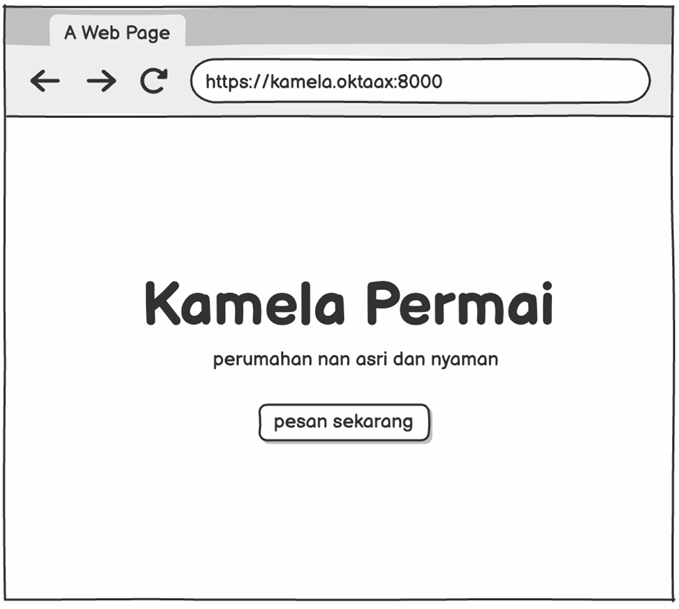
\includegraphics[width=0.75\linewidth]{Wireframe/Landing Page.png}
            \caption{Perancangan \textit{Interface Home}}
        \end{figure}
        
        \item Perancangan \textit{Interface Login}
        \par Perancangan \textit{interface Login} berguna untuk mengakses Sistem Presensi Karyawan yang terdiri dari \textit{Username, password} dan \textit{Login}.
        \begin{figure}
            \centering
            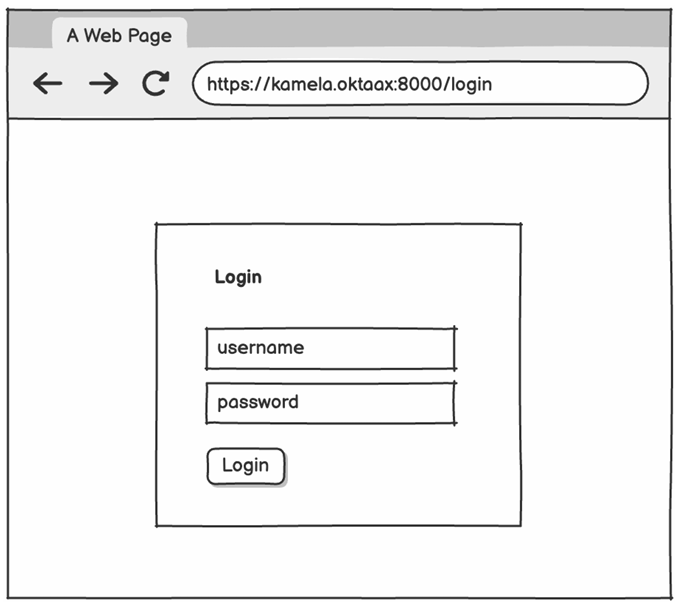
\includegraphics[width=0.75\linewidth]{Wireframe/Login.png}
            \caption{Perancangan \textit{Interface Login}}
        \end{figure}
        
        \item Perancangan \textit{Interface Dashboard}
        \par Berikut perancangan Interface Dashboard dapat dilihat pada gambar berikut.
        \begin{figure}
            \centering
            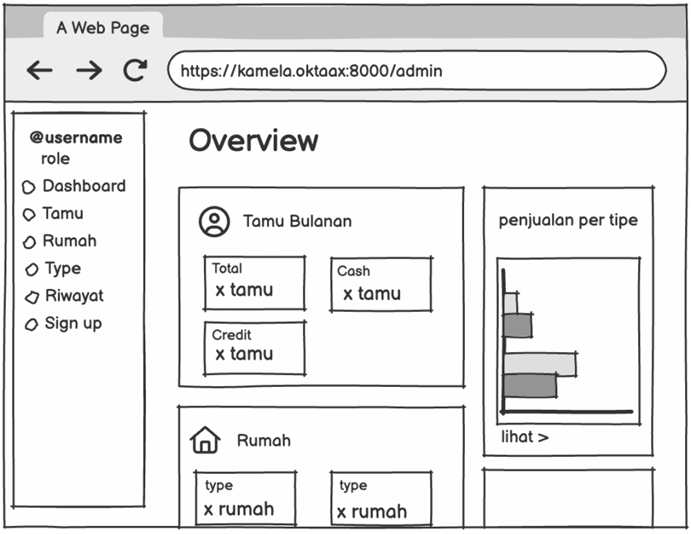
\includegraphics[width=0.75\linewidth]{Wireframe/Dashboard.png}
            \caption{Perancangan \textit{Interface Dashboard}}
        \end{figure}
        
        \item Perancangan \textit{Interface Data Rumah}
        \par Berikut perancangan \textit{Interface Data Rumah} dapat dilihat pada gambar berikut.
        \begin{figure}
            \centering
            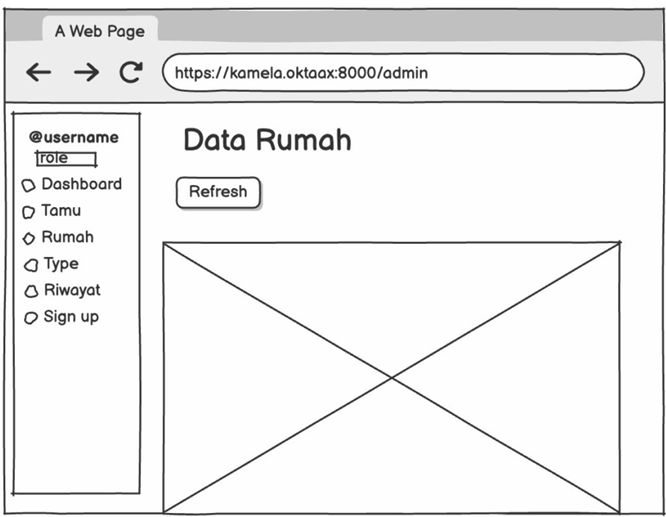
\includegraphics[width=0.75\linewidth]{Wireframe/Data Rumah.png}
            \caption{Perancangan \textit{Interface Data Rumah}}
        \end{figure}
        
        \item Perancangan \textit{Interface} Data Tamu
        \par Berikut adalah perancangan \textit{Interface} Data Tamu.
        \begin{figure}
            \centering
            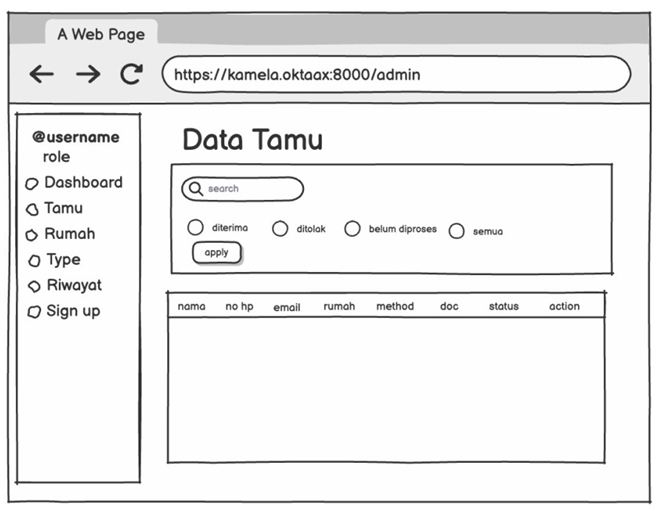
\includegraphics[width=0.75\linewidth]{Wireframe/Data Tamu.png}
            \caption{Perancangan \textit{Interface} Data Tamu}
        \end{figure}
        
        \item Perancangan \textit{Interface} Data Riwayat Pemesanan
        \par Berikut adalah perancangan \textit{Interface} Data Riwayat Pemesanan.
        \begin{figure}
            \centering
            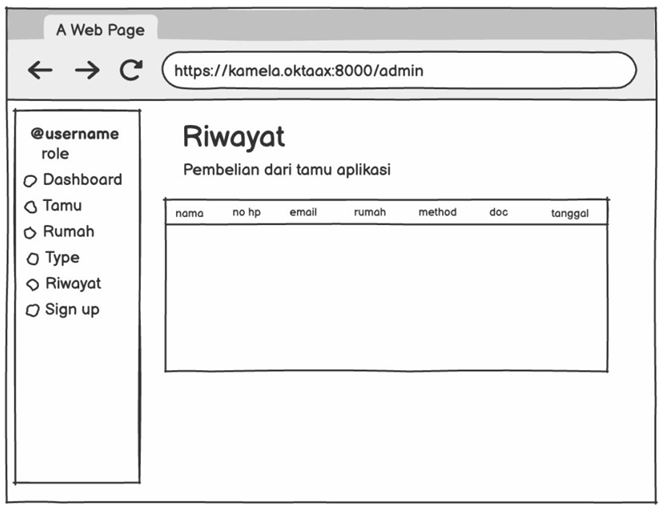
\includegraphics[width=0.75\linewidth]{Wireframe/Riwayat Pemesanan.png}
            \caption{Perancangan \textit{Interface} Data Riwayat Pemesanan}
        \end{figure}
        
        \item Perancangan \textit{Interface} Data Type
        \par Berikut adalah perancangan \textit{Interface} Data Type.
        \begin{figure}
            \centering
            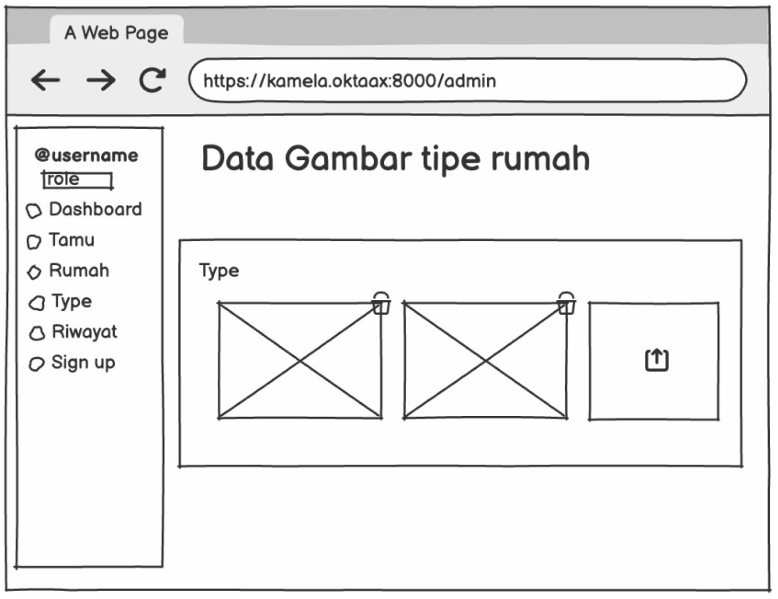
\includegraphics[width=0.75\linewidth]{Wireframe/Data Tipe.png}
            \caption{Perancangan \textit{Interface} Data Type}
        \end{figure}
        
        \item Perancangan \textit{Interface} Harga
        \par Berikut adalah perancangan \textit{Interface} Harga.
        \begin{figure}
            \centering
            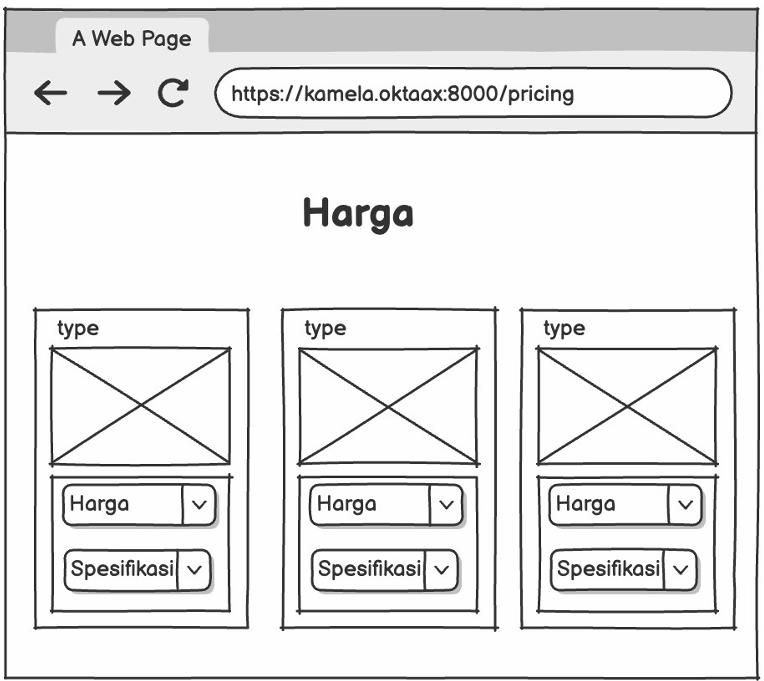
\includegraphics[width=0.75\linewidth]{Wireframe/Harga.png}
            \caption{Perancangan \textit{Interface} Harga}
        \end{figure}
        
        \item Perancangan \textit{Interface} Halaman Gallery
        \par Berikut adalah perancangan \textit{Interface} Halaman Gallery.
        \begin{figure}
            \centering
            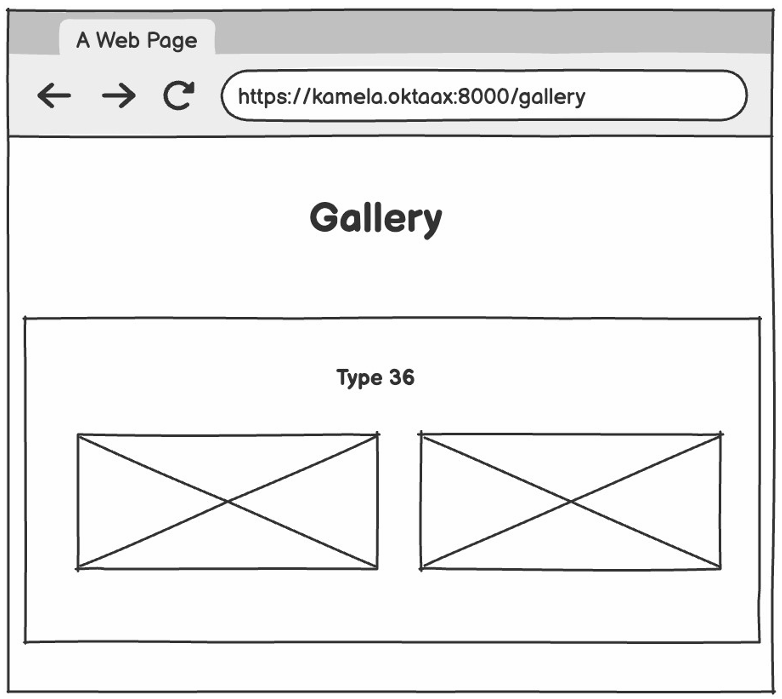
\includegraphics[width=0.75\linewidth]{Wireframe/Gallery.png}
            \caption{Perancangan \textit{Interface} Halaman Gallery}
        \end{figure}
        
        \item Perancangan \textit{Interface} Panduan
        \par Berikut adalah perancangan \textit{Interface} Panduan.
        \begin{figure}
            \centering
            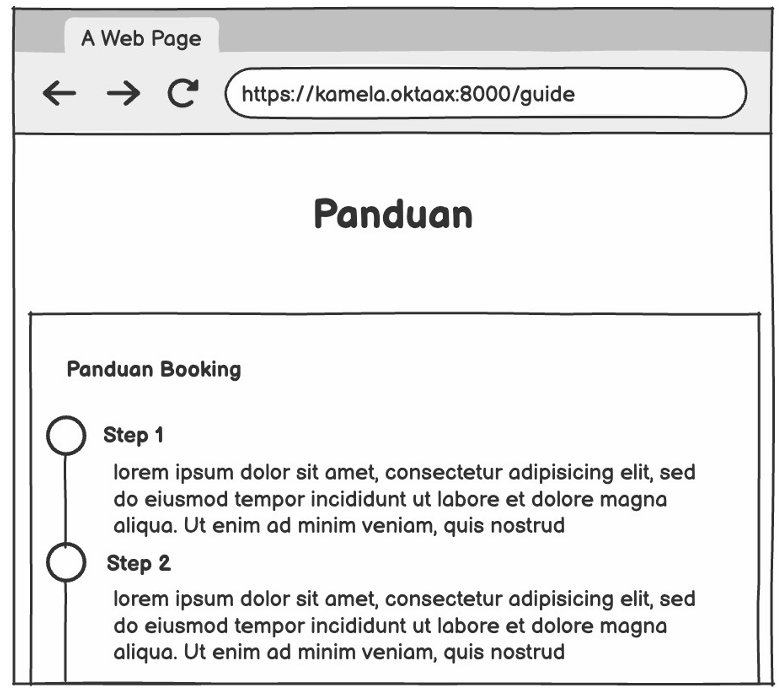
\includegraphics[width=0.72\linewidth]{Wireframe/Panduan.png}
            \caption{Perancangan \textit{Interface} Panduan}
        \end{figure}
        
        \item Perancangan \textit{Interface Site Plan}
        \par Berikut adalah perancangan \textit{Interface Site Plan}.
        \begin{figure}
            \centering
            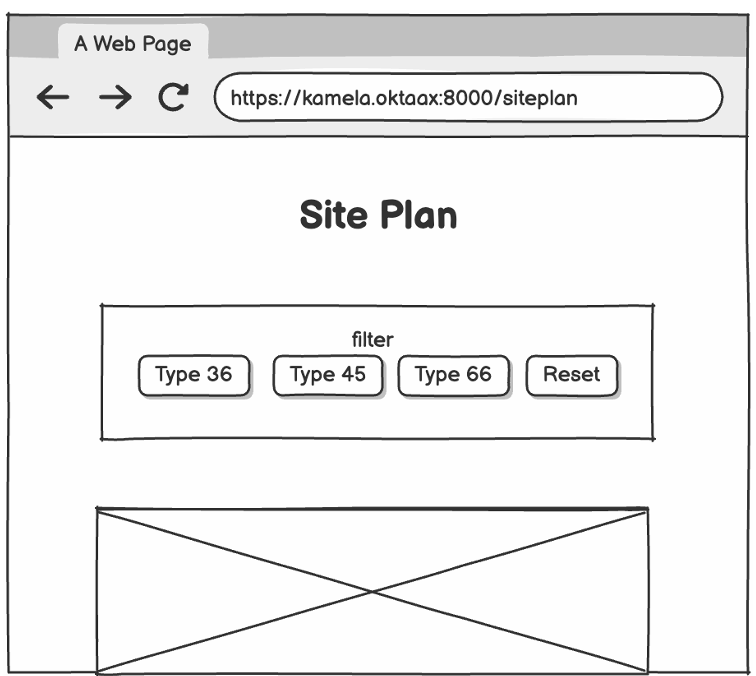
\includegraphics[width=0.72\linewidth]{Wireframe/Site Plan.png}
            \caption{Perancangan \textit{Interface Site Plan.}}
        \end{figure}

    \end{enumerate}
% -----------------------------------------------------------------------------%
\section{Hasil}

\subsection{Implementasi Sitem}
\par Implementasi sistem merupakan bentuk asli sistem yang dibuat berdasarkan rancangan interface yang telah dibuat sebelumnya, sehingga akan menampilkan bentuk sistem secara keseluruhannya. Tahap implementasi merupakan tahap meletakkan sistem supaya siap untuk dioperasikan, tahap ini termasuk juga kegiatan menulis kode program jika tidak digunakan paket perangkat lunak aplikasi dan pengetesan program. Berikut adalah beberapa hasil implementasi sistem.

\begin{enumerate}
    \item Halaman \textit{Home}
    \par Tampilan halaman home  dapat dilihat pada gambar berikut:

    \begin{figure}
        \centering
        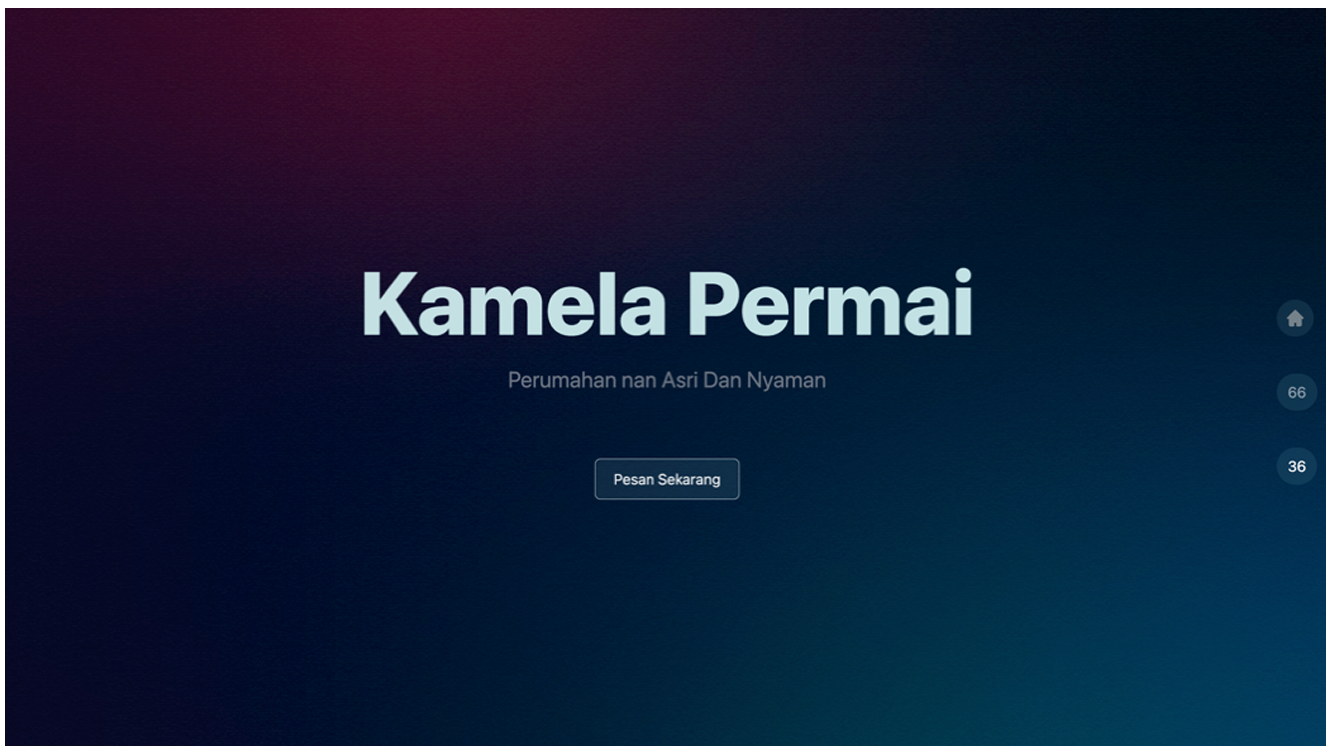
\includegraphics[width=0.75\linewidth]{Implementasi/Home.png}
        \caption{Halaman \textit{Home}}
    \end{figure}
    
    \item Halaman \textit{Login}
    \par Berikut adalah tampilan login, untuk megakses sistem penggua diharuskan mengisi \textit{username} dan \textit{password} terlebih dahulu dapat dilihat pada gambar berikut.
    \begin{figure}
        \centering
        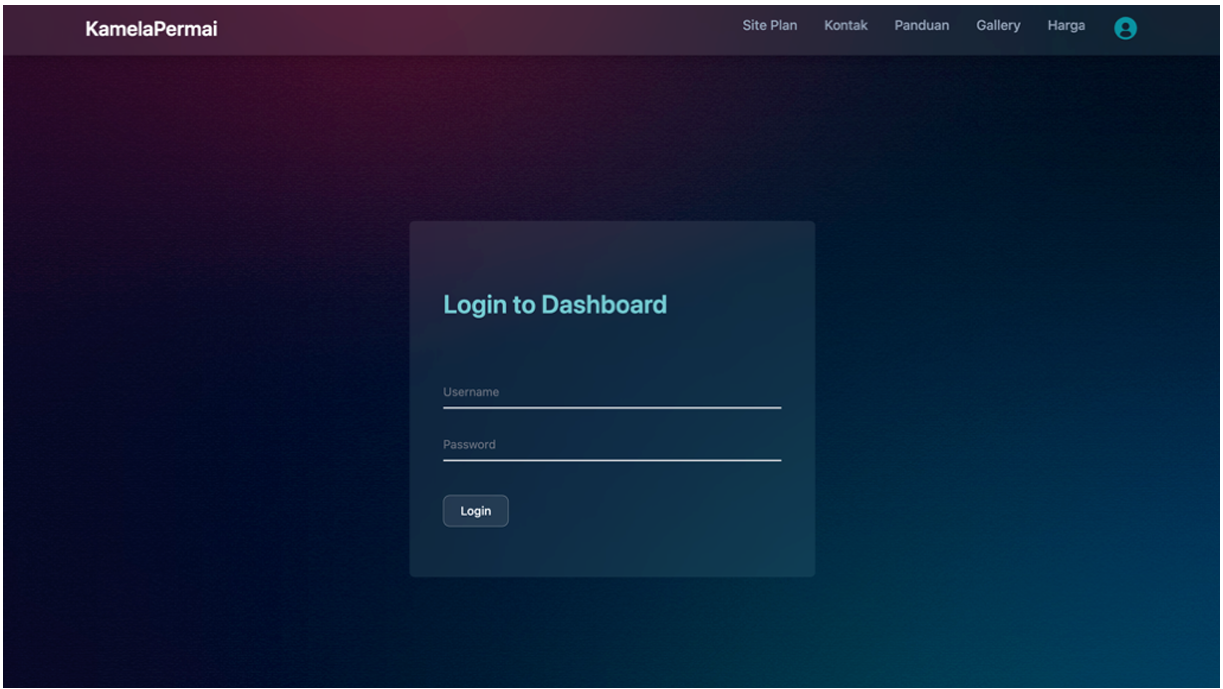
\includegraphics[width=0.75\linewidth]{Implementasi/Login.png}
        \caption{Halaman \textit{Login}}
    \end{figure}
    
    \item Halaman Dashboard Admin
    \par Berikut halaman dashboard yang menampilkan beberapa fitur yang tersedia pada sistem dapat dilihat pada gambar berikut.
    \begin{figure}
        \centering
        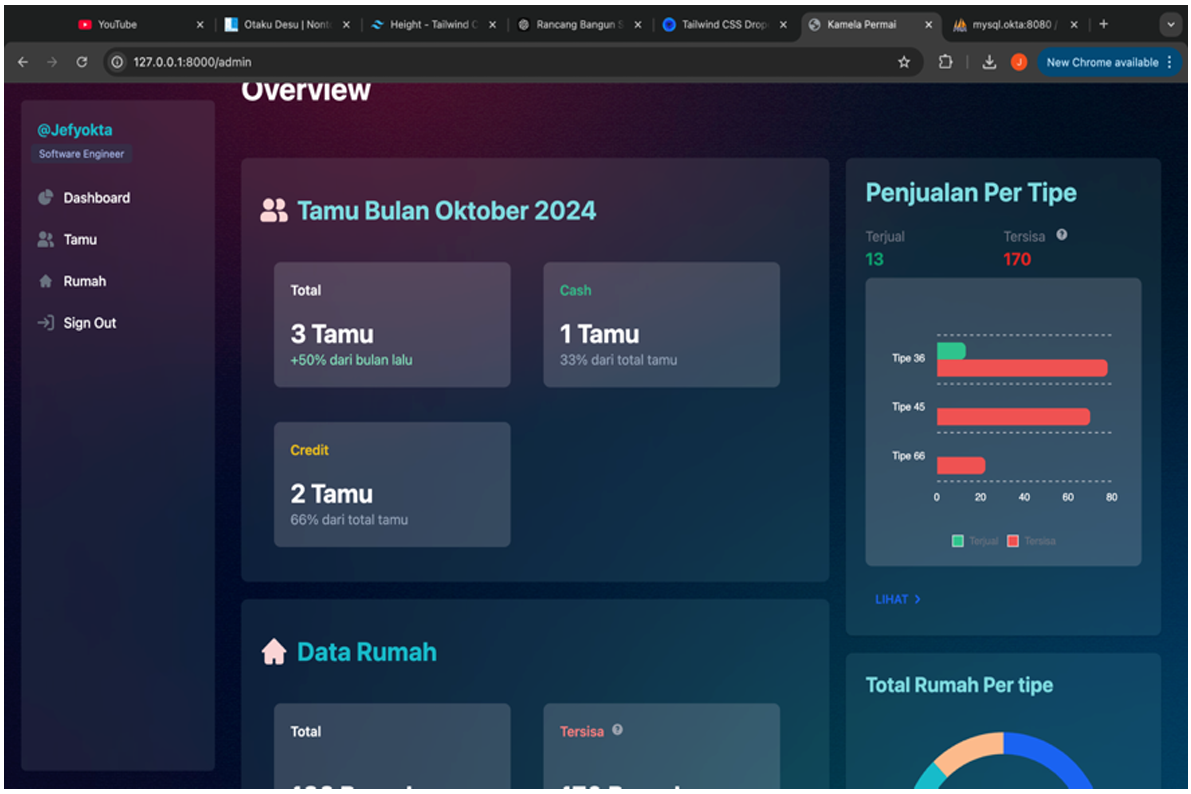
\includegraphics[width=0.75\linewidth]{Implementasi/Dashboard Admin.png}
        \caption{Halaman Dashboard Admin}
    \end{figure}
    
    \item Halaman Data Rumah
    \par Pada gambar dibawah merupakan gambar halaman untuk melakukan pengubahan pada data rumah serta mengubah status ketersediaanya yang dapat dilihat pada gambar berikut.
    \begin{figure}
        \centering
        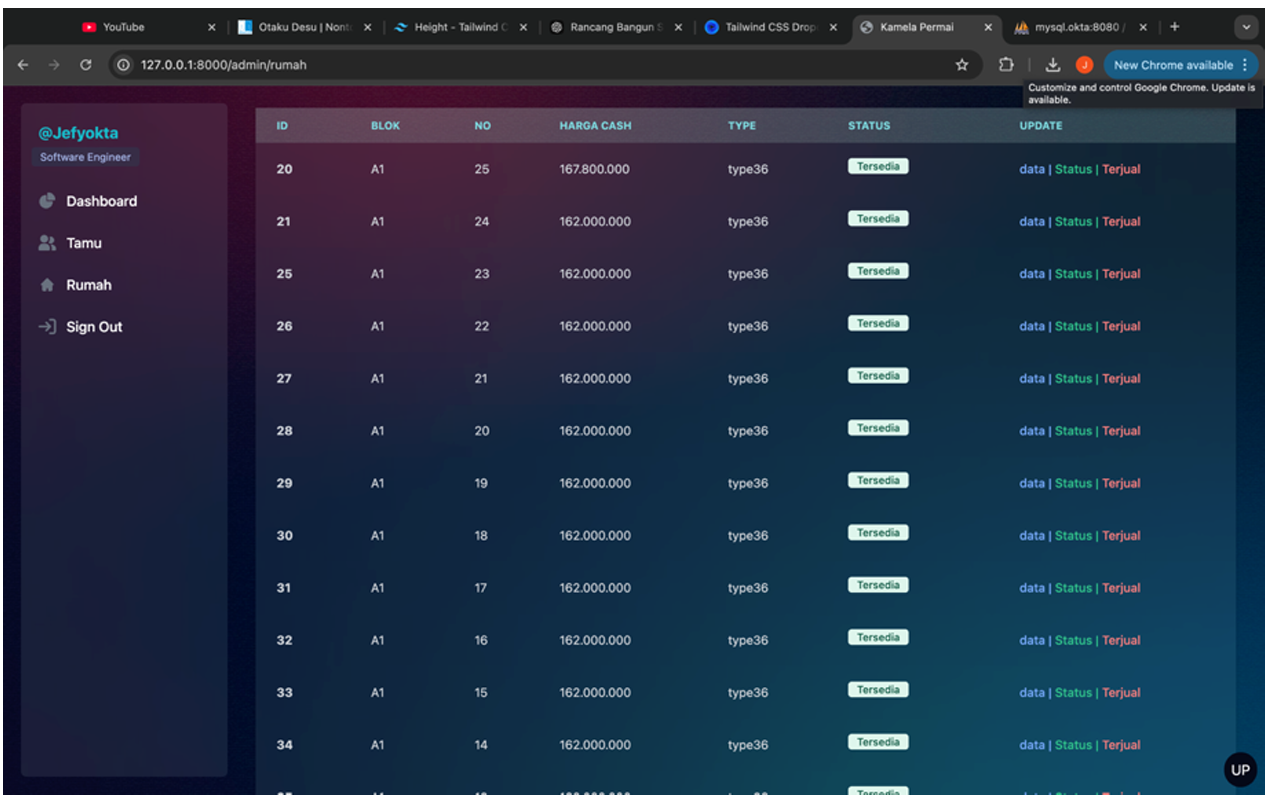
\includegraphics[width=0.75\linewidth]{Implementasi/Data Rumah.png}
        \caption{Halaman Data Rumah}
    \end{figure}

	 \begin{figure}
	        \centering
	        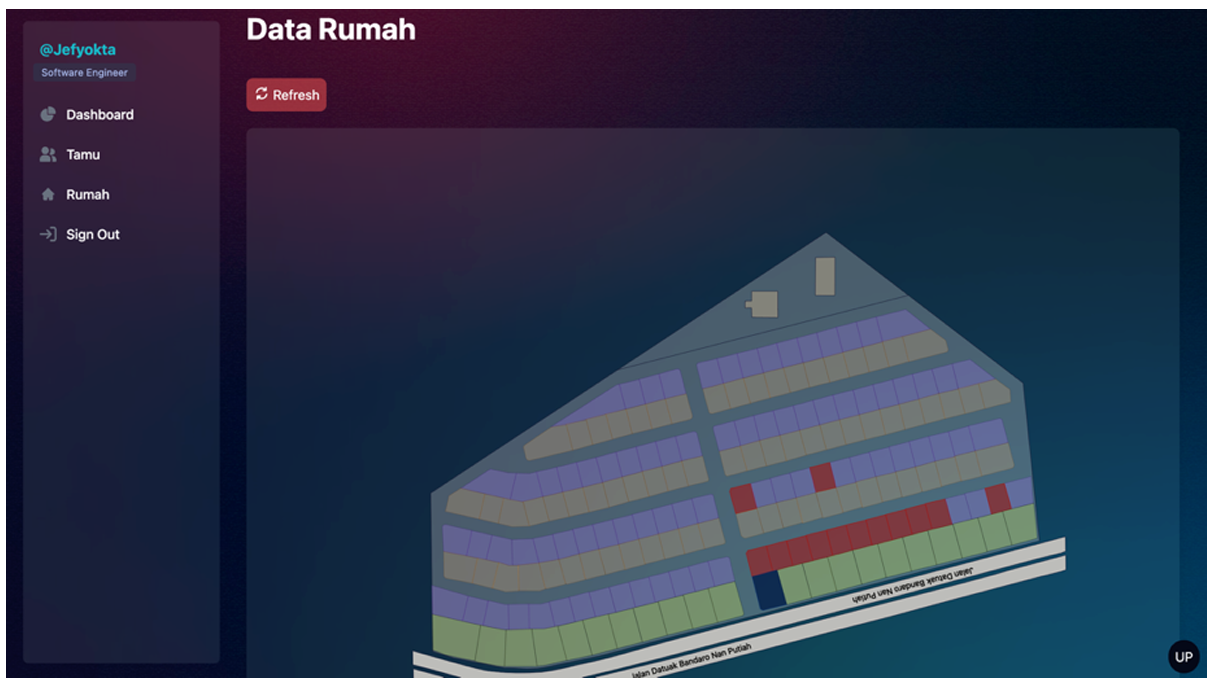
\includegraphics[width=0.75\linewidth]{Implementasi/Data Rumah 2.png}
	        \caption{Halaman Data Rumah 2}
	    \end{figure}
    
    \item Halaman Data Tamu
    \par Pada halaman data tamu ini terdapat no, nama, nomor telepon, email, dokumen dan aksi. Pada halaman ini admin dapat menerima pemesanan atau menghapusnya dapat dilihat pada gambar berikut.
    \begin{figure}
        \centering
        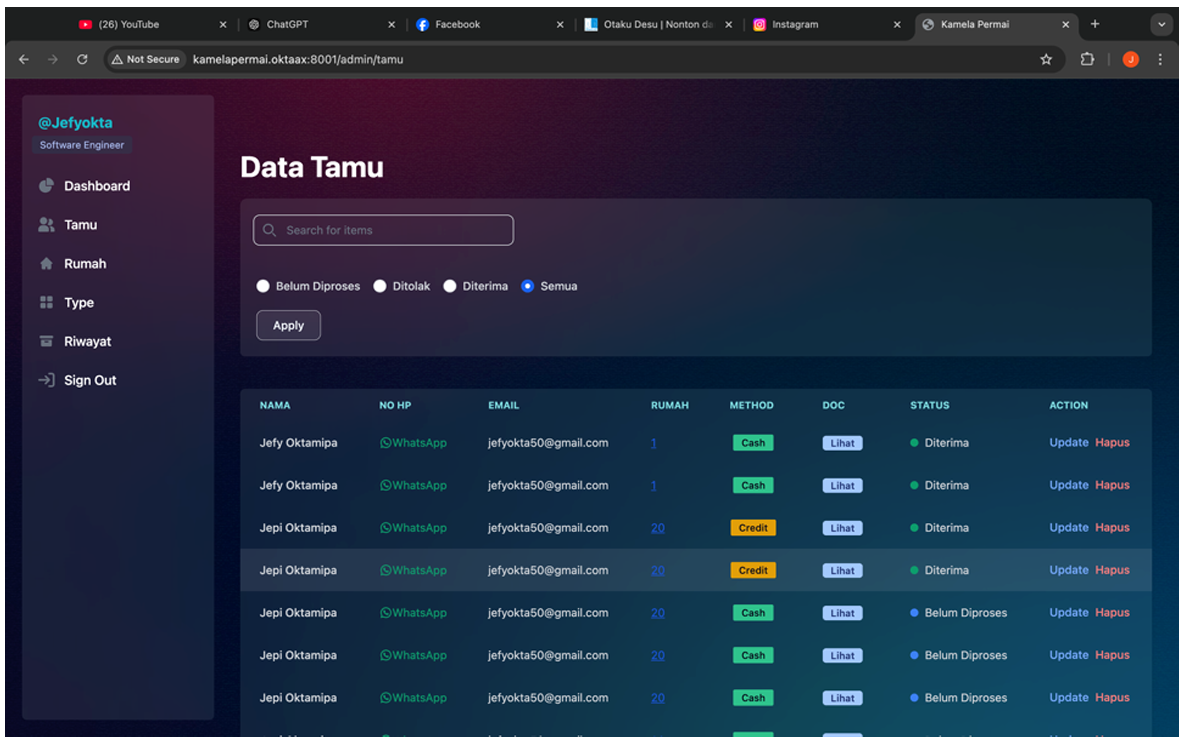
\includegraphics[width=0.75\linewidth]{Implementasi/Data Tamu.png}
        \caption{Halaman Data Tamu}
    \end{figure}
    
    \item Halaman Data Riwayat Pemesanan
    \par Pada halaman data riwayat terdapat data tamu yang berhasil booking. Admin dapat melihatnya seperti digambar berikut.
    \begin{figure}
        \centering
        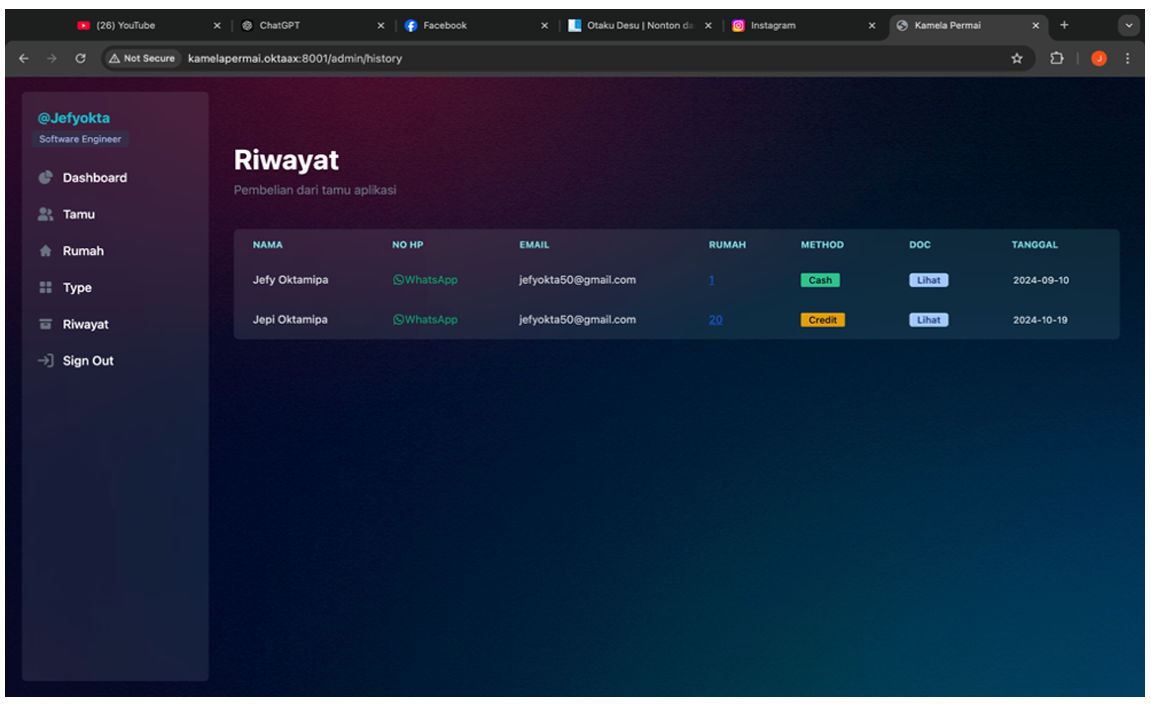
\includegraphics[width=0.75\linewidth]{Implementasi/Data Riwayat Pemesanan.png}
        \caption{Halaman Data Riwayat Pemesanan}
    \end{figure}
    
    \item Halaman Data \textit{Type}
    \par Pada halaman data \textit{Type} Terdapat gambar untuk setiap tipe yang dapat di tambah ataupun dihapus oleh admin. Dapat dilihat pada gambar berikut:.
    \begin{figure}
        \centering
        \includegraphics[width=0.75\linewidth]{Implementasi/Data Type.png}
        \caption{Halaman Data \textit{Type}}
    \end{figure}
    
    \item Halaman Harga
    \par Pada halaman harga terdapat harga cash, booking, cicilian dan spesifikasi setiap type nya yang dapat dilihat pada gambar berikut.
    \begin{figure}
        \centering
        \includegraphics[width=0.75\linewidth]{Implementasi/Harga.png}
        \caption{Halaman Harga}
    \end{figure}
    
    \item Halaman \textit{Gallery}
    \par Pada halaman gallery terdapat gambar setiap type yang sudah ditambahkan admin dan dapat dilihat oleh publik. Halaman dapat dilihat pada gambar berikut.
    \begin{figure}
        \centering
        \includegraphics[width=0.75\linewidth]{Implementasi/Gallery.png}
        \caption{Halaman \textit{Gallery}}
    \end{figure}
    
    \item Halaman Panduan
    \par Halaman ini berisi panduan untuk tamu yang ingin booking rumah secara cash atau credit. Halaman dapat dilihat pada gambar berikut.
    \begin{figure}
        \centering
        \includegraphics[width=0.75\linewidth]{Implementasi/Panduan.png}
        \caption{Halaman Panduan}
    \end{figure}
    
    \item Halaman \textit{Booking}
    \par Pada halaman ini, tamu yang sudah memilih rumah dapat mengisi form untuk pembookingan. Dapat dilihat pada gambar berikut.
    \begin{figure}
        \centering
        \includegraphics[width=0.75\linewidth]{Implementasi/Booking.png}
        \caption{Halaman \textit{Booking}}
    \end{figure}
    
\end{enumerate}

\subsection{Testing}
\par Dalam pengujian perangkat lunak terdapat berbagai metode yang bisa digunakan untuk melakukan pengujian, misalnya metode \textit{Black Box Testing}. \textit{Black Box Testing} merupakan salah satu metode pengujian yang berfokus pada spesifikasi fungsionalitas dari perangkat lunak. Pengujian ini memberikan gambaran atas sekumpulan kondisi masukan dan melakukan pengujian pada uraian pada fungsional program.
\par \textit{Black Box Testing} digunakan untuk mendeteksi permasalahan berikut:

\begin{enumerate}
\item Fungsi yang salah atau hilang.
\item Kesalahan pada interface.
\item Kesalahan struktur data dan basis data.
\item Kesalahan fungsi.
\item Kesalahan deklrasi dan terminasi.
\end{enumerate}

\par Berikut pengujian yang dilakukan menggunakan \textit{Black Box Testng} pada Sistem Pemesanan Perumahan Kamela Permai:

\renewcommand{\arraystretch}{1.2} % Atur jarak vertikal antar baris
\setlength{\tabcolsep}{4pt} % Atur padding horizontal antar kolom

\begin{scriptsize} % Ukuran teks lebih kecil untuk tabel
\begin{longtable}{|p{2.5cm}|>{\raggedright}p{4.5cm}|p{4cm}|p{1.5cm}|p{2cm}|}
    \caption{\textit{Black Box Testing}} \label{tab:hasil-pengujian} \\ \hline
    \textbf{Kasus Uji} & \textbf{Prosedur Pengujian} & \textbf{Keluaran yang Diharapkan} & \textbf{Hasil} & \textbf{Kesimpulan} \\ \hline
    \endfirsthead
    \hline
    \endfoot

    % Konten tabel
    Buka sistem & Buka \textit{website} menggunakan \textit{web browser} & Tampilan sistem & \checkmark & Diterima \\ \hline
    Login admin & Masukkan \textit{username} dan \textit{password} lalu klik login & Halaman admin & \checkmark & Diterima \\ \hline
    Booking & 
    - Buka halaman \textit{siteplan} \newline
    - Memilih rumah serta metode \newline
    - Mengisi formulir pemesanan &
    Pemesanan Berhasil & \checkmark & Diterima \\ \hline
    Menu tamu & Klik tamu & Menu tamu & \checkmark & Diterima \\ \hline
    Menu rumah & Klik rumah & Menu rumah & \checkmark & Diterima \\ \hline
    Menu type & Klik \textit{type} & Menampilkan data \textit{type} & \checkmark & Diterima \\ \hline
    Menu Logout & Klik logout & Sesi Berakhir & \checkmark & Diterima \\ \hline

\end{longtable}

\end{scriptsize}



\ifthenelse{\equal{\tipeta}{LAPORAN KERJA PRAKTEK}}{
  %-----------------------------------------------------------------------------------------------%
%
% % Oktober 2022
% Template Latex untuk Laporan Kerja Praktek Program Studi Sistem informasi ini
% Dikembangkan oleh Daffa Takratama Savra (daffatakratama13@gmail.com)

% Template ini dikembangkan dari template yang dibuat oleh Inggih Permana (inggihjava@gmail.com).

% Orang yang cerdas adalah orang yang paling banyak mengingat kematian.
%
%-----------------------------------------------------------------------------------------------%

%-----------------------------------------------------------------------------%
\chapter{\babLima}
% -----------------------------------------------------------------------------%
\section{Kesimpulan}
% -----------------------------------------------------------------------------%
\par Berdasarkan hasil kerja praktek saya yang berjudul Rancang Bangun Sistem Informasi Pemesanan Rumah (Perumahan Kamela Permai) , saya mendapat kesimpulan sebagai berikut:
\begin{enumerate}
\item Analisa sistem yang sedang berjalan perumahan Kamela Permau memiliki beberapa permasalahan dan hambatan dalam pemesanan rumahnya. Maka dengan adanya analisa usulan baru yaitu Sistem Informasi Pemesanan Perumahan akan menghasilkan solusi serta gambaran sistem yang lebih baik dan pemesanan rumah dapat dilakukan secara cepat dan efisien.
\item Dengan dibangunnya Sistem Informasi Pemesanan Perumahan ini dapat mempermudah jalannya pemesanan rumah di perumahan Kamela Permai.
\item Mengurangi biaya operasional dan memberikan kemudahan bagi pegawai untuk melihat data tamu tanpa harus disimpan secara fisik.
\end{enumerate}
% -----------------------------------------------------------------------------%
\section{Saran}
\par Saran yang membangun untuk kemajuan penelitian ini yaitu untuk penelitian selanjutnya diharapkan agar bisa membangun sebuah sistem yang telah yang memili fitur payment gateway agar pihak instansi lebih mudah untuk menerima pembayaran, karena pada sistem yang diusulkan sekarang ini sistem yang diberikan belum terintergrasi \textit{Payment Gateway}. Dan juga diharapkan agar bisa membangun sistem yang tampilannya lebih menarik dan mudah dimengerti. Semoga Sistem Informasi Pemesanan Perumahan ini pada tahap selanjutnya dapat dilakukan pengembangan dan implementasi menjadi sistem yang lebih baik dan sempurna terhadap Sistem Informasi Pemesanan Perumahan.
% -----------------------------------------------------------------------------%
  \ifthenelse{\equal{\bidangta}{SATU}}{
    \include{./konten/bab6}
  }{}
}{}

\bibliographystyle{apacite}
\renewcommand{\thepage}{}
\renewcommand{\bibname}{DAFTAR PUSTAKA}
\bibliography{konfigurasi/daftarpustaka}


\begin{appendix}

  \begin{appendices}
    \renewcommand{\appendixname}{LAMPIRAN}
    \renewcommand{\chaptername}{LAMPIRAN}
    \setcounter{page}{0}
%-----------------------------------------------------------------------------------------------%
%
% Oktober 2022
% Template Latex untuk Laporan Kerja Praktek Program Studi Sistem informasi ini
% Dikembangkan oleh Daffa Takratama Savra (daffatakratama13@gmail.com)

% Template ini dikembangkan dari template yang dibuat oleh Inggih Permana (inggihjava@gmail.com).

% Orang yang cerdas adalah orang yang paling banyak mengingat kematian.
%
%-----------------------------------------------------------------------------------------------%

%-----------------------------------------------------------------------------%
\prefikLampiran{A}
\renewcommand{\thepage}{A - \arabic{page}}
\chapter{Surat Izin Kerja Praktek}

\begin{figure}
        \centering
        \includegraphics[width=1.0\linewidth]{lampiran a.jpg}
    \end{figure}
% -----------------------------------------------------------------------------%


\setcounter{page}{1}
%-----------------------------------------------------------------------------------------------%
%
% % Oktober 2022
% Template Latex untuk Laporan Kerja Praktek Program Studi Sistem informasi ini
% Dikembangkan oleh Daffa Takratama Savra (daffatakratama13@gmail.com)

% Template ini dikembangkan dari template yang dibuat oleh Inggih Permana (inggihjava@gmail.com).

% Orang yang cerdas adalah orang yang paling banyak mengingat kematian.
%
%-----------------------------------------------------------------------------------------------%

%-----------------------------------------------------------------------------%
\prefikLampiran{A}

\renewcommand{\thepage}{B - \arabic{page}}
\chapter{Transkip Wawancara atau Hasil Observasi}

%-----------------------------------------------------------------------------%

\setcounter{page}{1}
%-----------------------------------------------------------------------------------------------%
%
% % Oktober 2022
% Template Latex untuk Laporan Kerja Praktek Program Studi Sistem informasi ini
% Dikembangkan oleh Daffa Takratama Savra (daffatakratama13@gmail.com)

% Template ini dikembangkan dari template yang dibuat oleh Inggih Permana (inggihjava@gmail.com).

% Orang yang cerdas adalah orang yang paling banyak mengingat kematian.
%
%-----------------------------------------------------------------------------------------------%

%-----------------------------------------------------------------------------%
\prefikLampiran{A}

\renewcommand{\thepage}{B - \arabic{page}}
\chapter{Dokumentasi}

\begin{figure}
        \centering
        \includegraphics[width=0.75\linewidth]{lampiran c.jpg}
    \end{figure}
%-----------------------------------------------------------------------------%

\setcounter{page}{1}
%-----------------------------------------------------------------------------------------------%
%
% % Oktober 2022
% Template Latex untuk Laporan Kerja Praktek Program Studi Sistem informasi ini
% Dikembangkan oleh Daffa Takratama Savra (daffatakratama13@gmail.com)

% Template ini dikembangkan dari template yang dibuat oleh Inggih Permana (inggihjava@gmail.com).

% Orang yang cerdas adalah orang yang paling banyak mengingat kematian.
%
%-----------------------------------------------------------------------------------------------%

%-----------------------------------------------------------------------------%
\prefikLampiran{A}

\renewcommand{\thepage}{C - \arabic{page}}
\chapter{Source Code/Interface/Materi Pengmas/Tutorial/Dll}
\begin{figure}
        \centering
        \includegraphics[width=0.75\linewidth]{lampiran d.png}
    \end{figure}
%-----------------------------------------------------------------------------%
  \end{appendices}
\end{appendix}

\include{./halamanbelakang/daftarRiwayatHidup}

\end{document}